% Mini research note for trust-region Newton and preconditioning.
\documentclass[11pt]{article}
% Shared preamble for the research-note series.
% Create note-specific content in the per-note directory; keep common macros here.
\usepackage[margin=1in]{geometry}
\usepackage[T1]{fontenc}
\usepackage[utf8]{inputenc}
\usepackage{amsmath,amssymb}
\usepackage{booktabs,longtable,array}
\usepackage{graphicx}
\usepackage{float}
\usepackage{enumitem}
\usepackage{xcolor}
\usepackage{hyperref}
\usepackage{caption}
\usepackage{titlesec}
\hypersetup{colorlinks=true, linkcolor=blue!60!black, urlcolor=blue!60!black, citecolor=blue!60!black}
\setlist[itemize]{leftmargin=1.25em, itemsep=0.2em, topsep=0.3em}
\setlist[enumerate]{leftmargin=1.4em, itemsep=0.2em, topsep=0.3em}
\setlength{\parindent}{0pt}
\setlength{\parskip}{0.6em}
\newcommand{\statusbox}[2]{%
  \noindent\fcolorbox{black}{gray!10}{%
    \parbox{\dimexpr\linewidth-2\fboxsep-2\fboxrule\relax}{%
      \textbf{Status:} #1\\#2
    }%
  }
}

% Shared notation helpers for the research-note series.
\newcommand{\Jlin}{J}
\newcommand{\Jphys}{J_{\mathrm{phys}}}
\newcommand{\Jsurf}{J_{\mathrm{surf}}}
\newcommand{\JdB}{J_{\mathrm{dB}}}
\newcommand{\phiopt}{\phi_{\mathrm{opt}}}
\newcommand{\sigmathreedb}{\sigma_{3\mathrm{dB}}}
\newcommand{\Nt}{N_t}
\newcommand{\Nphi}{N_{\phi}}
\newcommand{\Lfiber}{L}
\newcommand{\Pcont}{P}
\newcommand{\band}{\mathcal{B}_{\mathrm{Raman}}}
\newcommand{\todoitem}[1]{\textcolor{red!70!black}{\textbf{TODO:} #1}}


\title{Trust-Region Newton Methods in a Saddle-Dominated Raman Landscape}
\author{Fiber Raman Suppression Project}
\date{Evidence snapshot: 2026-04-26}

\begin{document}
\maketitle

\begin{abstract}
This note asks whether second-order optimization should replace the default
first-order Raman-suppression workflow. The answer is useful but mostly
negative: trust-region Newton methods are excellent diagnostics for curvature,
but they did not become the default optimizer for this Raman objective. The
main reason is that the local quadratic model often sees strong negative
curvature, so cold-start runs collapse before accepting useful steps. After
gauge-safe preconditioning and bounded continuation tests, the dispersion
preconditioner gave a small localized benefit, but not a broad result. The
best practical lesson is that continuation supplies the path; trust-region
Newton can refine and diagnose that path, but it does not replace it.
\end{abstract}

\section*{Claim Status}
\statusbox{established diagnostic result; closed as a default replacement}{The
trust-region implementation is scientifically useful and technically honest
after the preconditioner and gauge-projection fixes. The evidence does not
support using it as the default Raman optimizer. Preconditioning alone does
not rescue bad cold starts, and the best dispersion-preconditioned gains were
too localized to justify keeping this as an active Raman-suppression branch.}

\section{Question and Thesis}

The baseline optimizer uses L-BFGS: it follows gradients and builds a cheap
low-memory curvature approximation. This note studies a more direct
second-order question:
\begin{center}
\emph{Can Newton-like curvature information give better Raman suppression or
more reliable optimization?}
\end{center}

The motivation is reasonable. If the objective has a locally quadratic shape,
then Newton information should help identify the best step. But this project
does not see a clean convex bowl. The resolved Hessian spectra around strong
optimized points have both positive and negative eigenvalues, so the landscape
is saddle-like. That changes the role of Newton methods. They become good
for diagnosing why the optimizer is stuck, but they are not automatically good
at finding a better phase mask from a poor starting point.

The current thesis is:
\[
    \text{trust-region Newton is a microscope, not the main engine.}
\]
It exposes curvature and failure modes clearly. The engine that still matters
most is continuation: move through easier problems into harder ones while
carrying a good phase profile forward.

\subsection*{Intuition Check}

L-BFGS asks, ``which downhill direction should I try next?'' Trust-region
Newton asks, ``if I locally approximate the objective by a quadratic bowl, what
step should I trust?'' The problem is that the local shape is often not a bowl.
It is more like a mountain pass: downhill in some directions and uphill in
others. In that setting, a Newton step can be mathematically informative but
experimentally unreliable unless the starting point is already on a good path.

\section{Common Setup}

The controlled field is still a phase-shaped input spectrum,
\[
    u_\omega(0;\phi)=u_{\omega,0}\exp(i\phi(\omega)).
\]
After propagation through the fiber, the physical Raman objective is the
Raman-band energy fraction
\[
    \Jphys(\phi)
    =
    \frac{
    \sum_{\omega_k\in\band}|u_{\omega_k}(L;\phi)|^2\,\Delta\omega
    }{
    \sum_k |u_{\omega_k}(L;\phi)|^2\,\Delta\omega
    }.
\]
The propagation model follows the usual generalized nonlinear Schrodinger
equation simulation stack for nonlinear fiber optics
\cite{agrawal2019,dudley2006,hult2007}. The baseline first-order optimizer is
L-BFGS \cite{liu1989,nocedal2006}. This note keeps the same physics objective
but changes the local optimization method.

\subsection*{Intuition Check}

The physics problem did not change. We are still trying to find a spectral
phase that keeps energy out of the Raman-shifted band. The only new question
is whether using Hessian-vector products makes the optimizer smarter.

\begin{figure}[H]
\centering
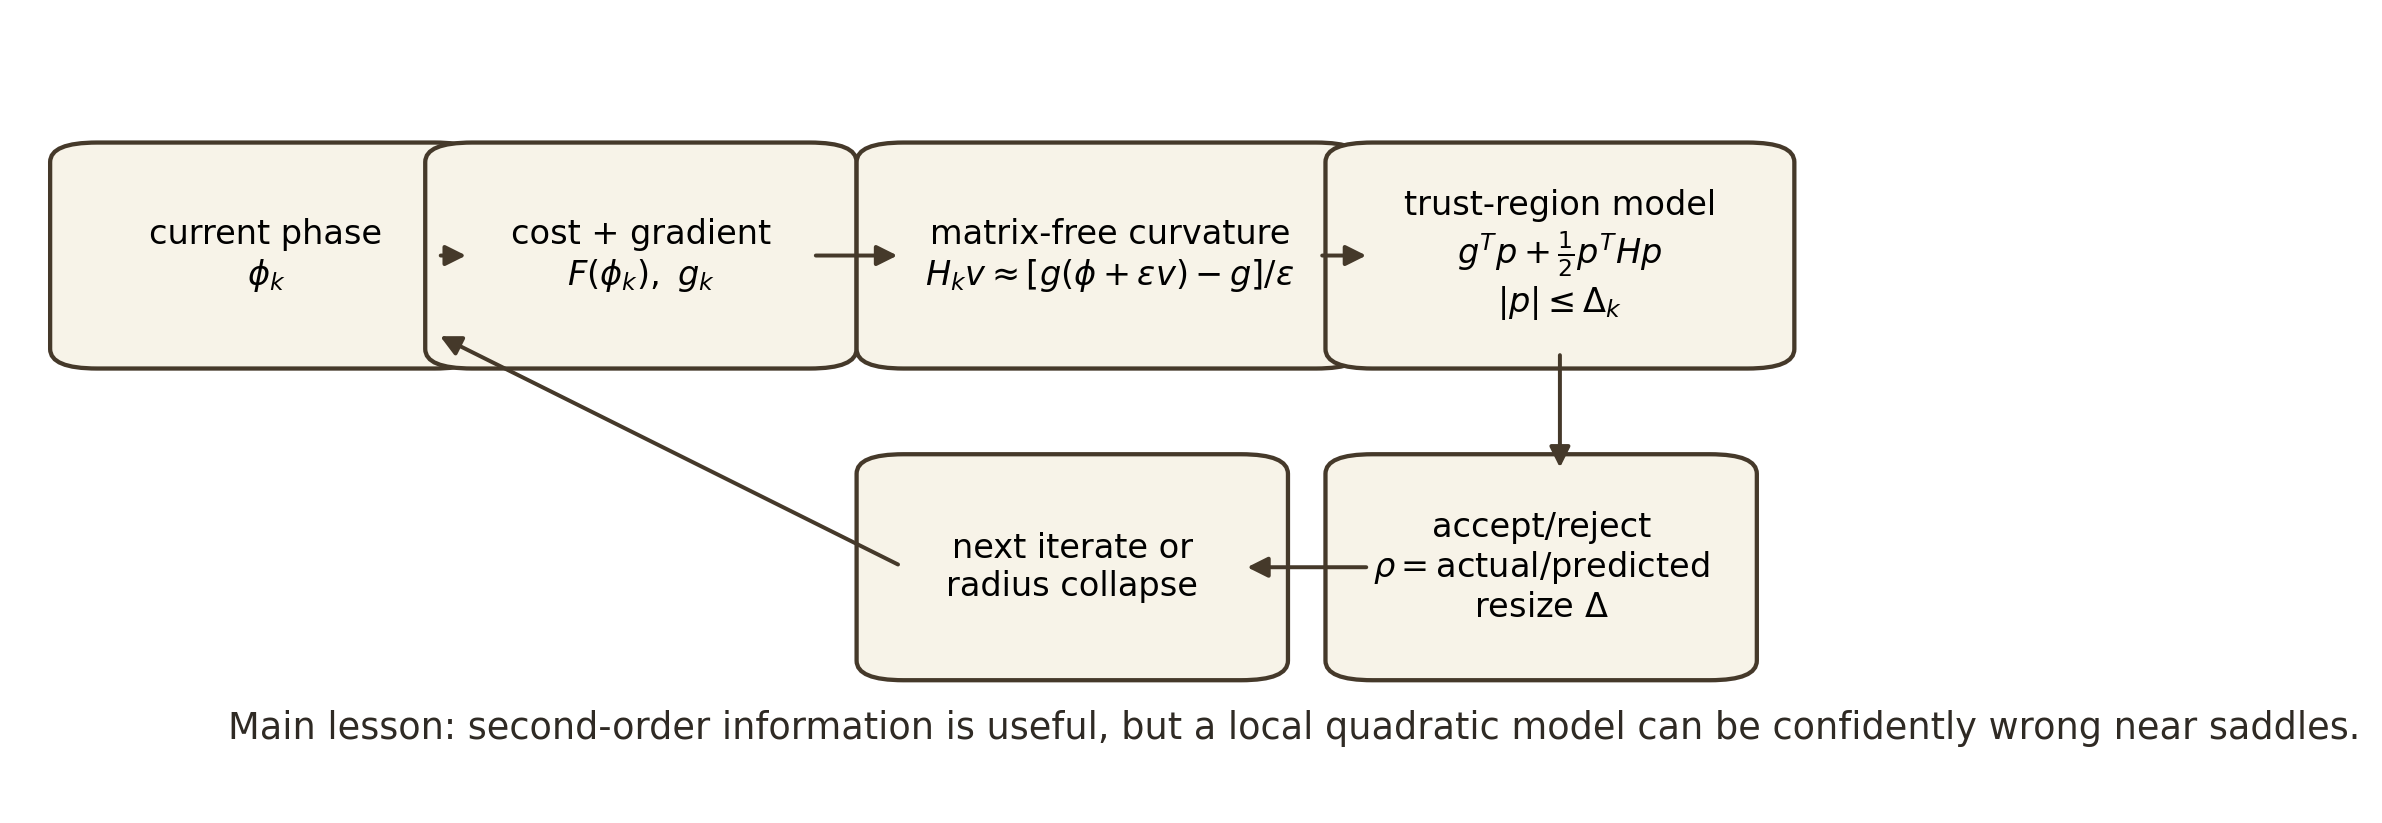
\includegraphics[width=0.96\linewidth]{figures/trust_region_workflow_diagram.png}
\caption{Trust-region workflow. The optimizer builds a local quadratic model
from the current cost, gradient, and Hessian-vector products. A trial step is
accepted only if the real forward simulation agrees well enough with the
quadratic prediction.}
\end{figure}

\section{Trust-Region Math}

Let \(F(\phi)\) be the scalar objective seen by the optimizer. At iteration
\(k\), define
\[
    g_k=\nabla F(\phi_k),
    \qquad
    H_k=\nabla^2 F(\phi_k).
\]
A Newton method approximates the objective near \(\phi_k\) by
\[
    m_k(p)=F(\phi_k)+g_k^T p+\frac{1}{2}p^T H_k p.
\]
The trust-region step solves the bounded quadratic problem
\[
    \min_p \; g_k^T p+\frac{1}{2}p^T H_k p
    \quad
    \text{subject to}
    \quad
    \|p\|_2 \leq \Delta_k,
\]
where \(\Delta_k\) is the radius of the region where we trust the quadratic
model.

After proposing \(p_k\), the optimizer compares predicted improvement to real
improvement:
\[
    \rho_k
    =
    \frac{F(\phi_k)-F(\phi_k+p_k)}
    {m_k(0)-m_k(p_k)}.
\]
If \(\rho_k\) is large enough, the step is accepted. If \(\rho_k\) is small or
negative, the step is rejected and the trust radius shrinks. The implementation
uses the standard trust-region thresholds
\[
    \rho < 0.25 \Rightarrow \Delta \leftarrow 0.25\|p\|,
    \qquad
    \rho > 0.75 \text{ and boundary step} \Rightarrow
    \Delta \leftarrow \min(2\Delta,\Delta_{\max}).
\]

\subsection*{Intuition Check}

The trust radius is a safety belt. A Newton model may be accurate very close
to the current phase mask but wrong far away. If a trial step improves the
real simulation as much as the model predicted, the optimizer trusts a larger
neighborhood. If the trial step fails, the optimizer becomes more cautious.

\section{Steihaug-CG and Negative Curvature}

The full Hessian is too large to build explicitly in the main simulations, so
the trust-region subproblem is solved with truncated conjugate gradient, often
called Steihaug-CG \cite{steihaug1983,nocedal2006}. This only needs products
\(H_k v\), not the matrix \(H_k\) itself.

The important saddle-specific rule is:
\[
    d^T H_k d \leq 0
    \quad
    \Rightarrow
    \quad
    \text{negative curvature detected.}
\]
When this happens, the inner solve stops and moves to the boundary of the
trust region in that direction. This is mathematically correct: in a direction
with negative curvature, the local quadratic model keeps decreasing as the
step grows, so the constrained best step sits on the boundary.

The Hessian-vector product is computed by finite differencing gradients,
\[
    H(\phi)v
    \approx
    \frac{\nabla F(\phi+\epsilon v)-\nabla F(\phi)}{\epsilon},
\]
with an adaptive \(\epsilon\) chosen from the current gradient and vector
norms. This is matrix-free but not free: each HVP costs extra gradient work.

\subsection*{Intuition Check}

Negative curvature is not a small numerical inconvenience. It means the
``bowl'' picture is wrong. The surface is bending downward in at least one
direction. That is why the cold-start runs can keep proposing boundary steps
that look good to the quadratic model but fail in the real simulation.

\section{Gauge Projection}

Phase-only Raman suppression has directions that do not change the physical
Raman energy ratio in the usual way. A constant phase mostly changes global
phase, and a linear phase in frequency mostly shifts the pulse in time. These
are gauge-like directions. If they are not handled carefully, curvature
diagnostics can waste effort on directions that are not meaningful control
degrees of freedom.

The optimizer projects gradients, Hessian-vector inputs, Hessian-vector
outputs, and preconditioned residuals into the gauge-complement subspace:
\[
    v_{\perp}=(I-P_{\mathcal{G}})v,
    \qquad
    \mathcal{G}=\operatorname{span}\{1,\omega-\bar{\omega}\}.
\]
Here \(P_{\mathcal{G}}\) is the least-squares projector onto constant and
linear-in-frequency phase directions. A gauge-leak guard checks that accepted
steps stay in this projected subspace.

\subsection*{Intuition Check}

This is a linear algebra cleanup step. If two phase changes are physically
equivalent for the Raman objective, we should not let the optimizer spend its
curvature budget distinguishing them. The projection says: remove the boring
global-phase/time-shift directions, then optimize the remaining shape.

\section{Preconditioning}

Preconditioning tries to make the inner CG problem easier by changing how
directions are scaled. In the preconditioned solve, the residual \(r\) is
mapped through an approximate inverse curvature operator,
\[
    z=M^{-1}r,
\]
and the CG search directions are built from \(z\) rather than directly from
\(r\). If \(M\approx H\) and \(M\) is stable, the inner solve can require fewer
iterations or propose better-scaled steps.

Three preconditioner ideas were tested in bounded cases:
\begin{itemize}
    \item \textbf{none:} identity scaling, the honest baseline.
    \item \textbf{dispersion:} frequency-dependent diagonal scaling
    \(d_i=1+\alpha(\omega_i/\max|\omega|)^2\).
    \item \textbf{DCT/reduced:} a low-dimensional cosine-basis Hessian
    approximation with a stabilizing shift.
\end{itemize}

The key implementation fix was that preconditioned residuals and directions
must be projected back into the gauge-complement space. Pointwise division by
a diagonal preconditioner does not commute with the gauge projection, so
without re-projection the preconditioner can create illegal gauge leakage.

\subsection*{Intuition Check}

Preconditioning is like changing units before doing geometry. If one direction
is naturally stiff and another is naturally soft, the optimizer can behave
better after rescaling. But rescaling cannot create a good optimization path
from nothing. In this project, the starting path mattered more than the
preconditioner.

\section{Implementation Surface}

\begin{center}
\small
\begin{tabular}{p{0.24\linewidth}p{0.66\linewidth}}
\toprule
\textbf{Component} & \textbf{Role} \\
\midrule
\texttt{core.jl}
& Steihaug-CG subproblem solver, trust-radius update, typed exit codes, and
subproblem result contract. \\
\texttt{optimize.jl}
& Raman trust-region outer loop, matrix-free HVP wrapper, acceptance ratio,
radius collapse checks, gauge projection, and standard result object. \\
\texttt{pcg.jl}
& Preconditioned CG solver with gauge-safe residual and direction projection. \\
\texttt{preconditioner.jl}
& Diagonal power, dispersion, and reduced DCT preconditioner factories. \\
\texttt{telemetry.jl}
& Per-iteration records: objective, gradient norm, radius, \(\rho\), accepted
flag, HVP counts, and curvature probes. \\
\bottomrule
\end{tabular}
\end{center}

All listed files are in \texttt{scripts/research/trust\_region/}.

The result object exposes a \texttt{minimizer} field so the normal standard
image pipeline can save phase diagnostics and spectral-evolution heat maps.

\section{Experimental Strategy}

The work was organized into four checks.

\begin{enumerate}
    \item \textbf{Hessian landscape check.} Probe the largest positive and
    most negative resolved Hessian eigenvalues at optimized reference points.
    The goal is to test whether the optimizer is near a convex minimum or a
    saddle-like stationary point.
    \item \textbf{Cold-start radius sweep.} Start from \(\phi=0\) and vary the
    initial trust radius \(\Delta_0\). If all radii collapse with no accepted
    steps, then the problem is not simply ``bad initial radius.''
    \item \textbf{Gauge-safe preconditioner reruns.} Compare no
    preconditioner, dispersion scaling, and reduced/DCT scaling after fixing
    the preconditioner wiring and gauge-projection issue.
    \item \textbf{Continuation-assisted ladder.} Solve an easier fiber length
    first, then move the phase mask to harder lengths and compare no
    preconditioner against dispersion preconditioning.
\end{enumerate}

\subsection*{Intuition Check}

This is not one giant benchmark. It is a sequence of sanity checks. First ask
what the landscape looks like. Then ask whether trust-region can leave the
control point. Then ask whether preconditioning helps. Finally ask whether it
helps when continuation has already supplied a reasonable path.

\section{Hessian Geometry Result}

\begin{figure}[H]
\centering
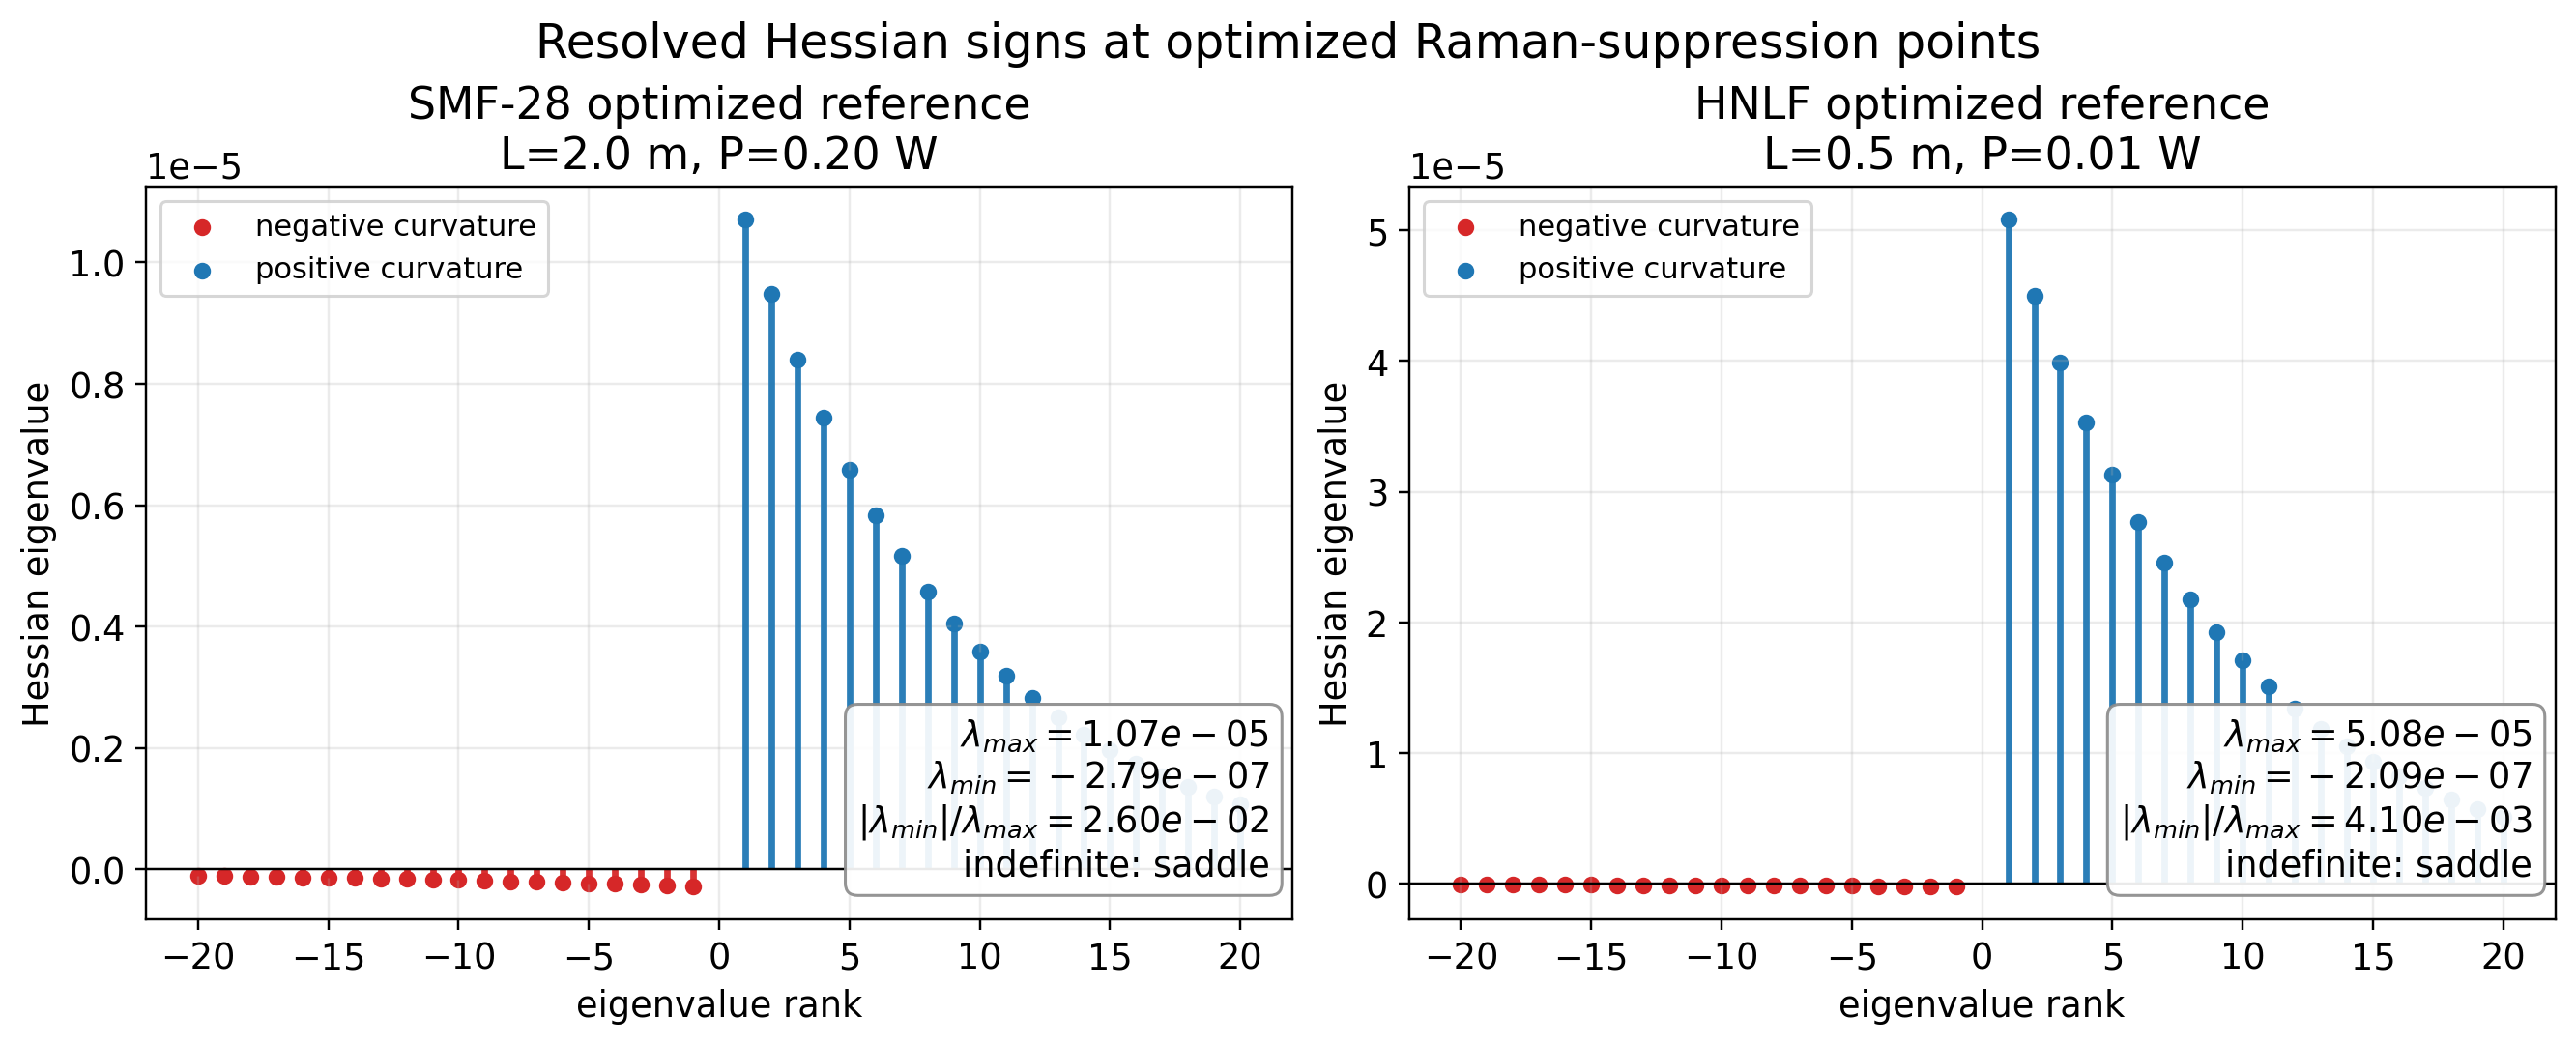
\includegraphics[width=0.94\linewidth]{figures/hessian_saddle_spectrum_clean.png}
\caption{Resolved Hessian signs at two optimized reference points. Both cases
show positive and negative curvature after gauge handling, so the local
geometry is saddle-like rather than a clean convex minimum.}
\end{figure}

At the optimized SMF-28 reference point, the largest resolved positive
eigenvalue was about \(1.07\times10^{-5}\), while the most negative resolved
eigenvalue was about \(-2.79\times10^{-7}\). At the optimized HNLF reference
point, the corresponding values were about \(5.08\times10^{-5}\) and
\(-2.09\times10^{-7}\). The negative directions are smaller than the stiff
positive directions, but they are not zero.

\subsection*{Intuition Check}

The solution is not sitting at the bottom of a smooth bowl. It is more like a
high-dimensional pass: some directions curve up, and some directions curve
down. That explains why a second-order method can detect a problem even when
the first-order gradient is already small.

\section{Cold-Start Radius Sweep}

\begin{figure}[H]
\centering
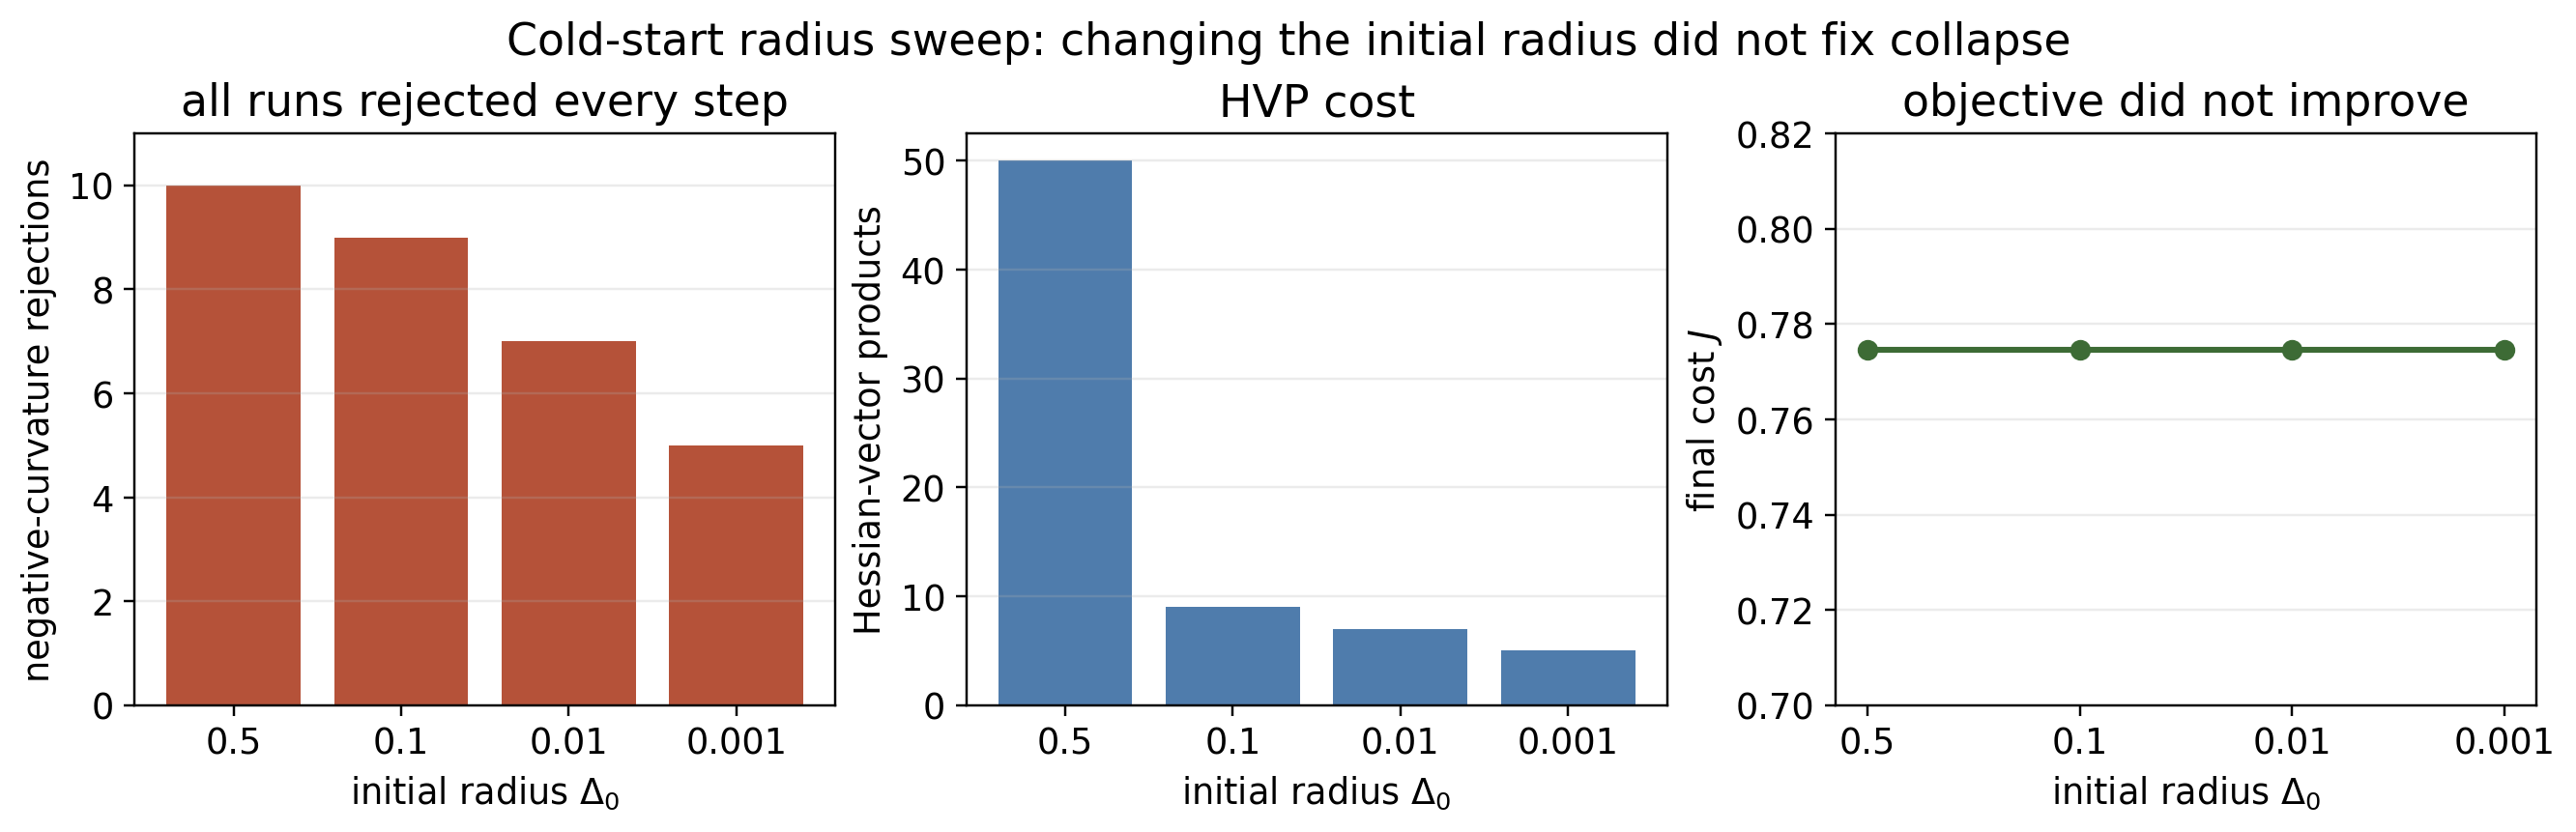
\includegraphics[width=0.96\linewidth]{figures/delta0_radius_collapse_summary.png}
\caption{Cold-start trust-region sweep on the canonical SMF-28 case. All
initial radii collapsed, no run accepted a step, and the objective stayed at
the unoptimized baseline value.}
\end{figure}

\begin{center}
\small
\begin{tabular}{ccccc}
\toprule
\(\Delta_0\) & exit & final \(J\) & accepted & negative-curvature rejections \\
\midrule
0.5   & radius collapse & \(7.746118\times10^{-1}\) & 0 & 10 \\
0.1   & radius collapse & \(7.746118\times10^{-1}\) & 0 & 9 \\
0.01  & radius collapse & \(7.746118\times10^{-1}\) & 0 & 7 \\
0.001 & radius collapse & \(7.746118\times10^{-1}\) & 0 & 5 \\
\bottomrule
\end{tabular}
\end{center}

The largest-radius run also measured strong local indefiniteness during the
collapse: \(\lambda_{\min}\approx-303.1\) and
\(\lambda_{\max}\approx547.4\). The absolute values are on the local objective
scale used by that trust-region run, not directly comparable to the reference
Hessian plot above. The sign pattern is the important part.

\subsection*{Intuition Check}

Changing the initial radius is like asking the optimizer to take a smaller or
larger first step. This sweep says the first-step size was not the real issue.
The local quadratic model itself was not giving acceptable real improvements
from the zero phase mask.

\clearpage
\section{Representative Result Pages}

Each page below pairs the phase diagnostic with the corresponding spectral
evolution heat map. The first page is the no-optimization reference.

\begin{figure}[p]
\centering
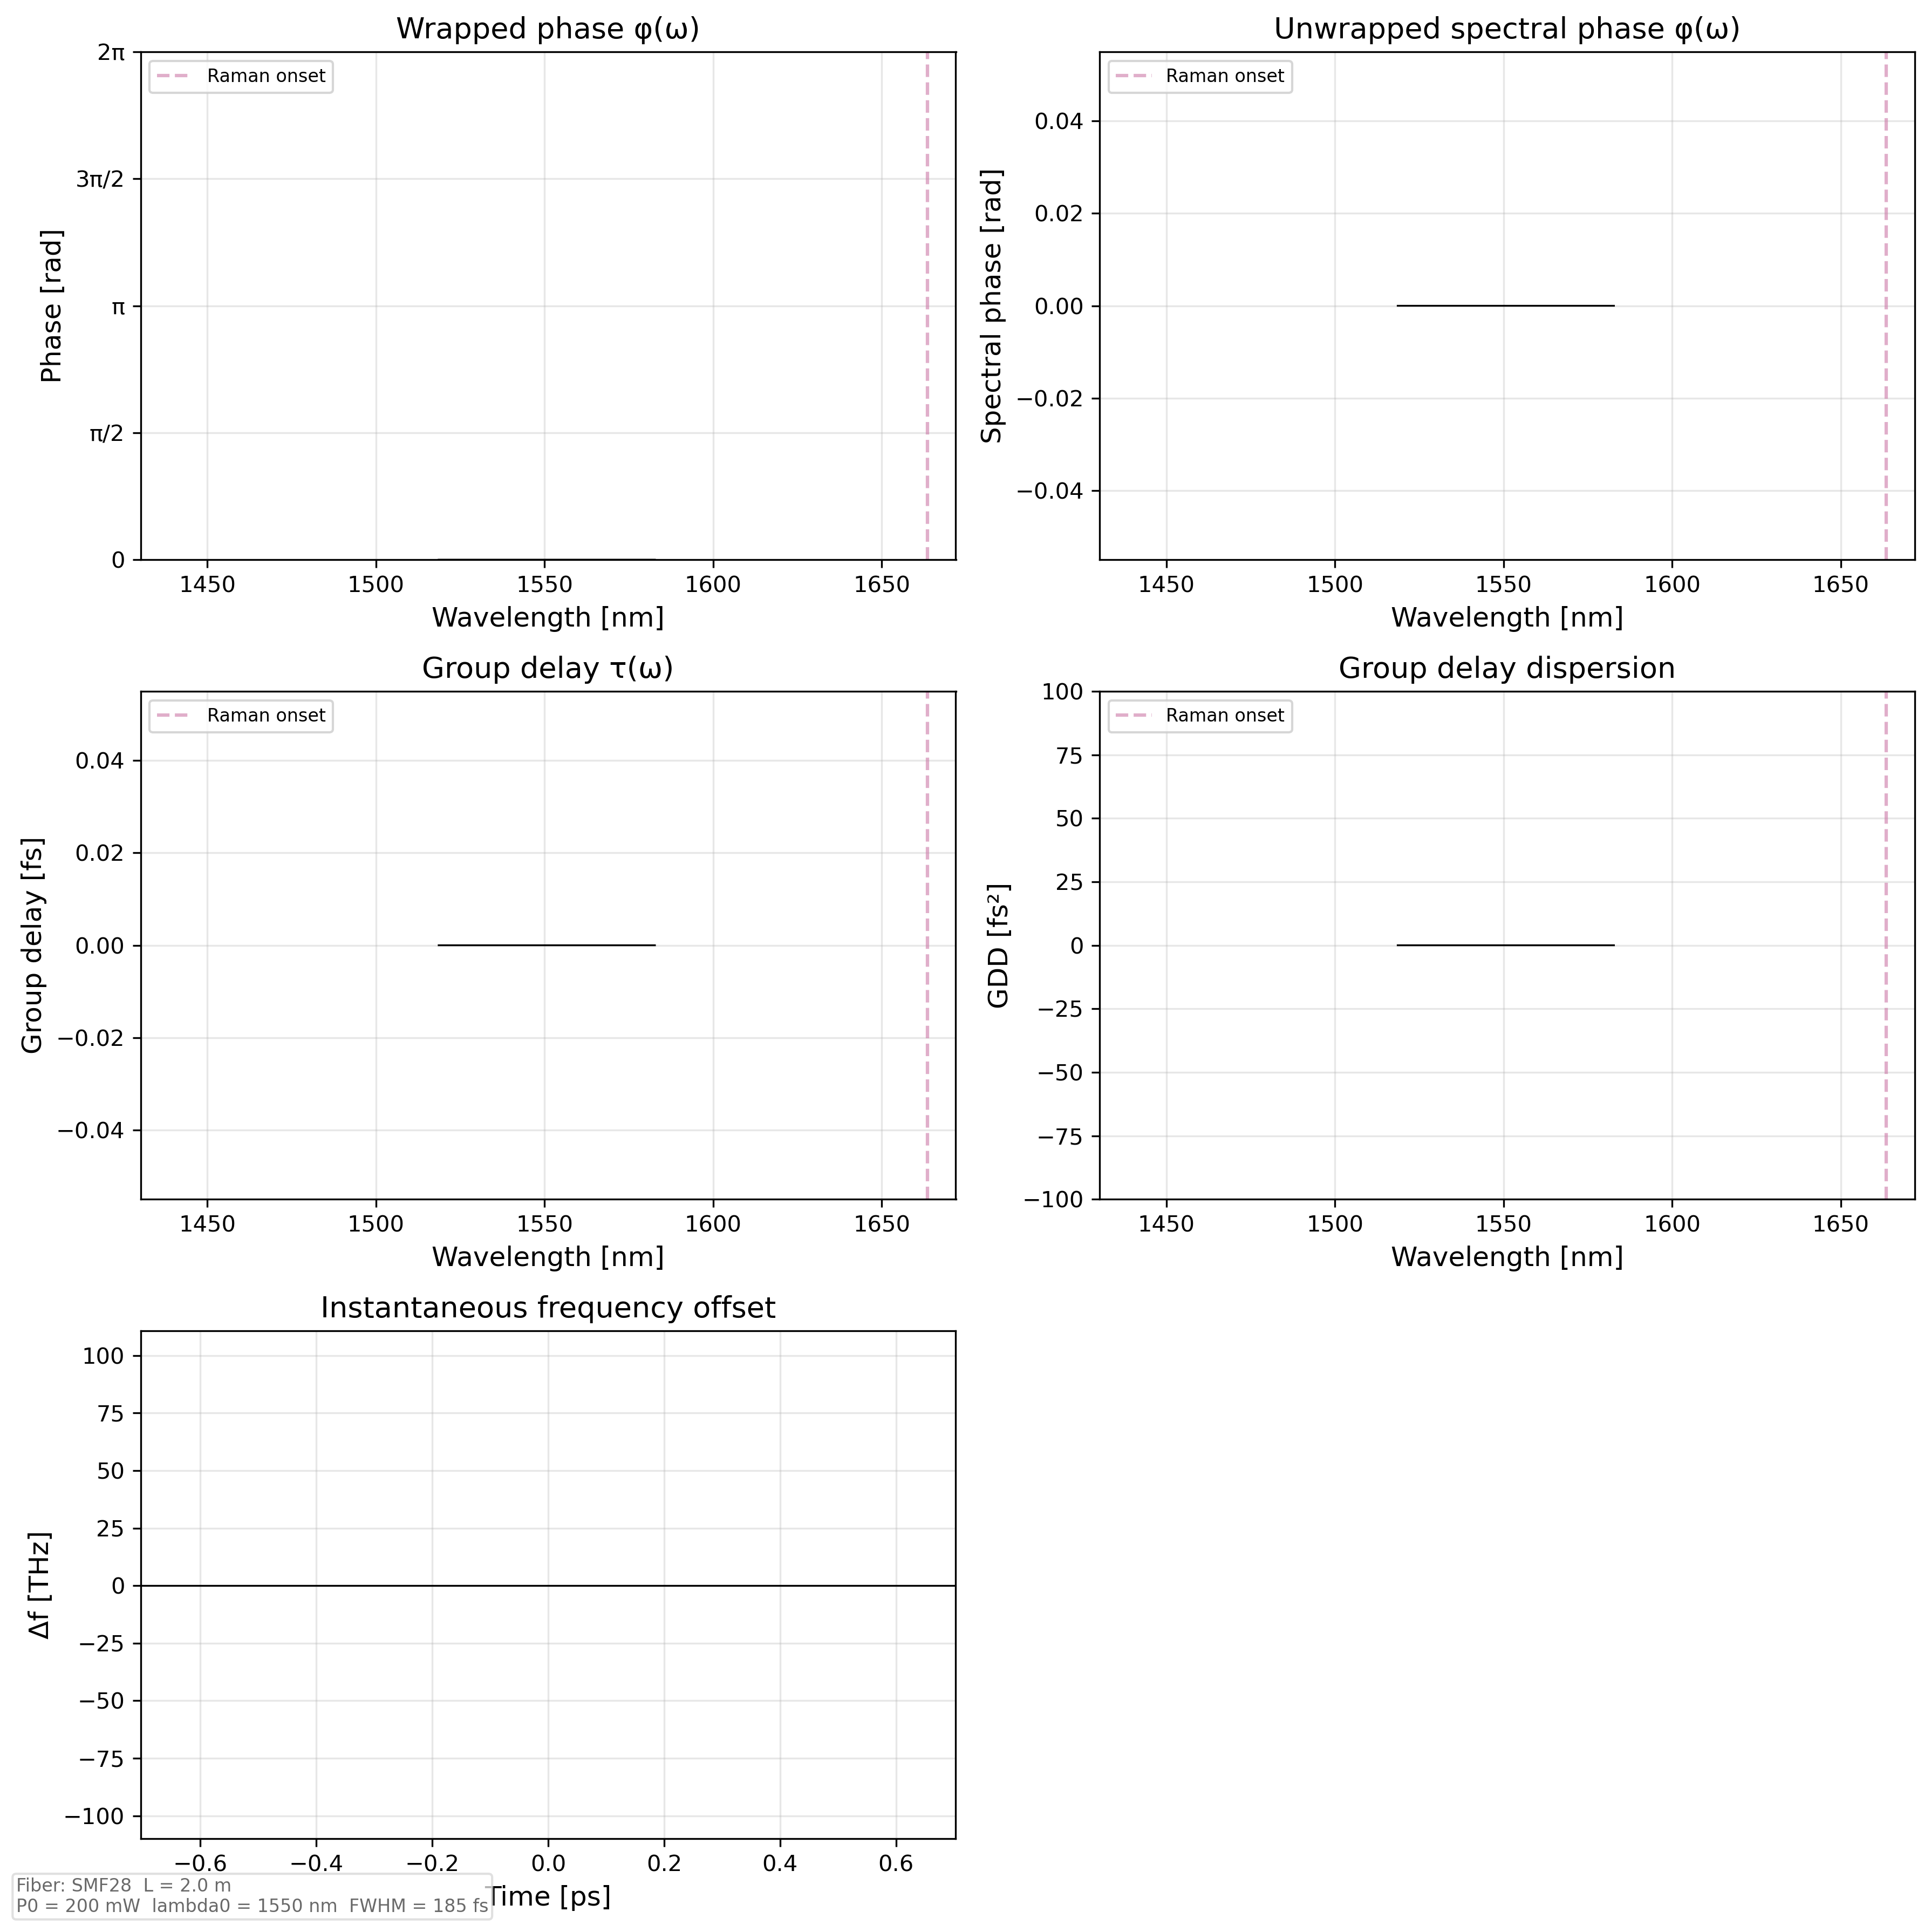
\includegraphics[height=0.48\textheight]{figures/control_no_optimization_phase_diagnostic.png}
\par\vspace{0.5em}
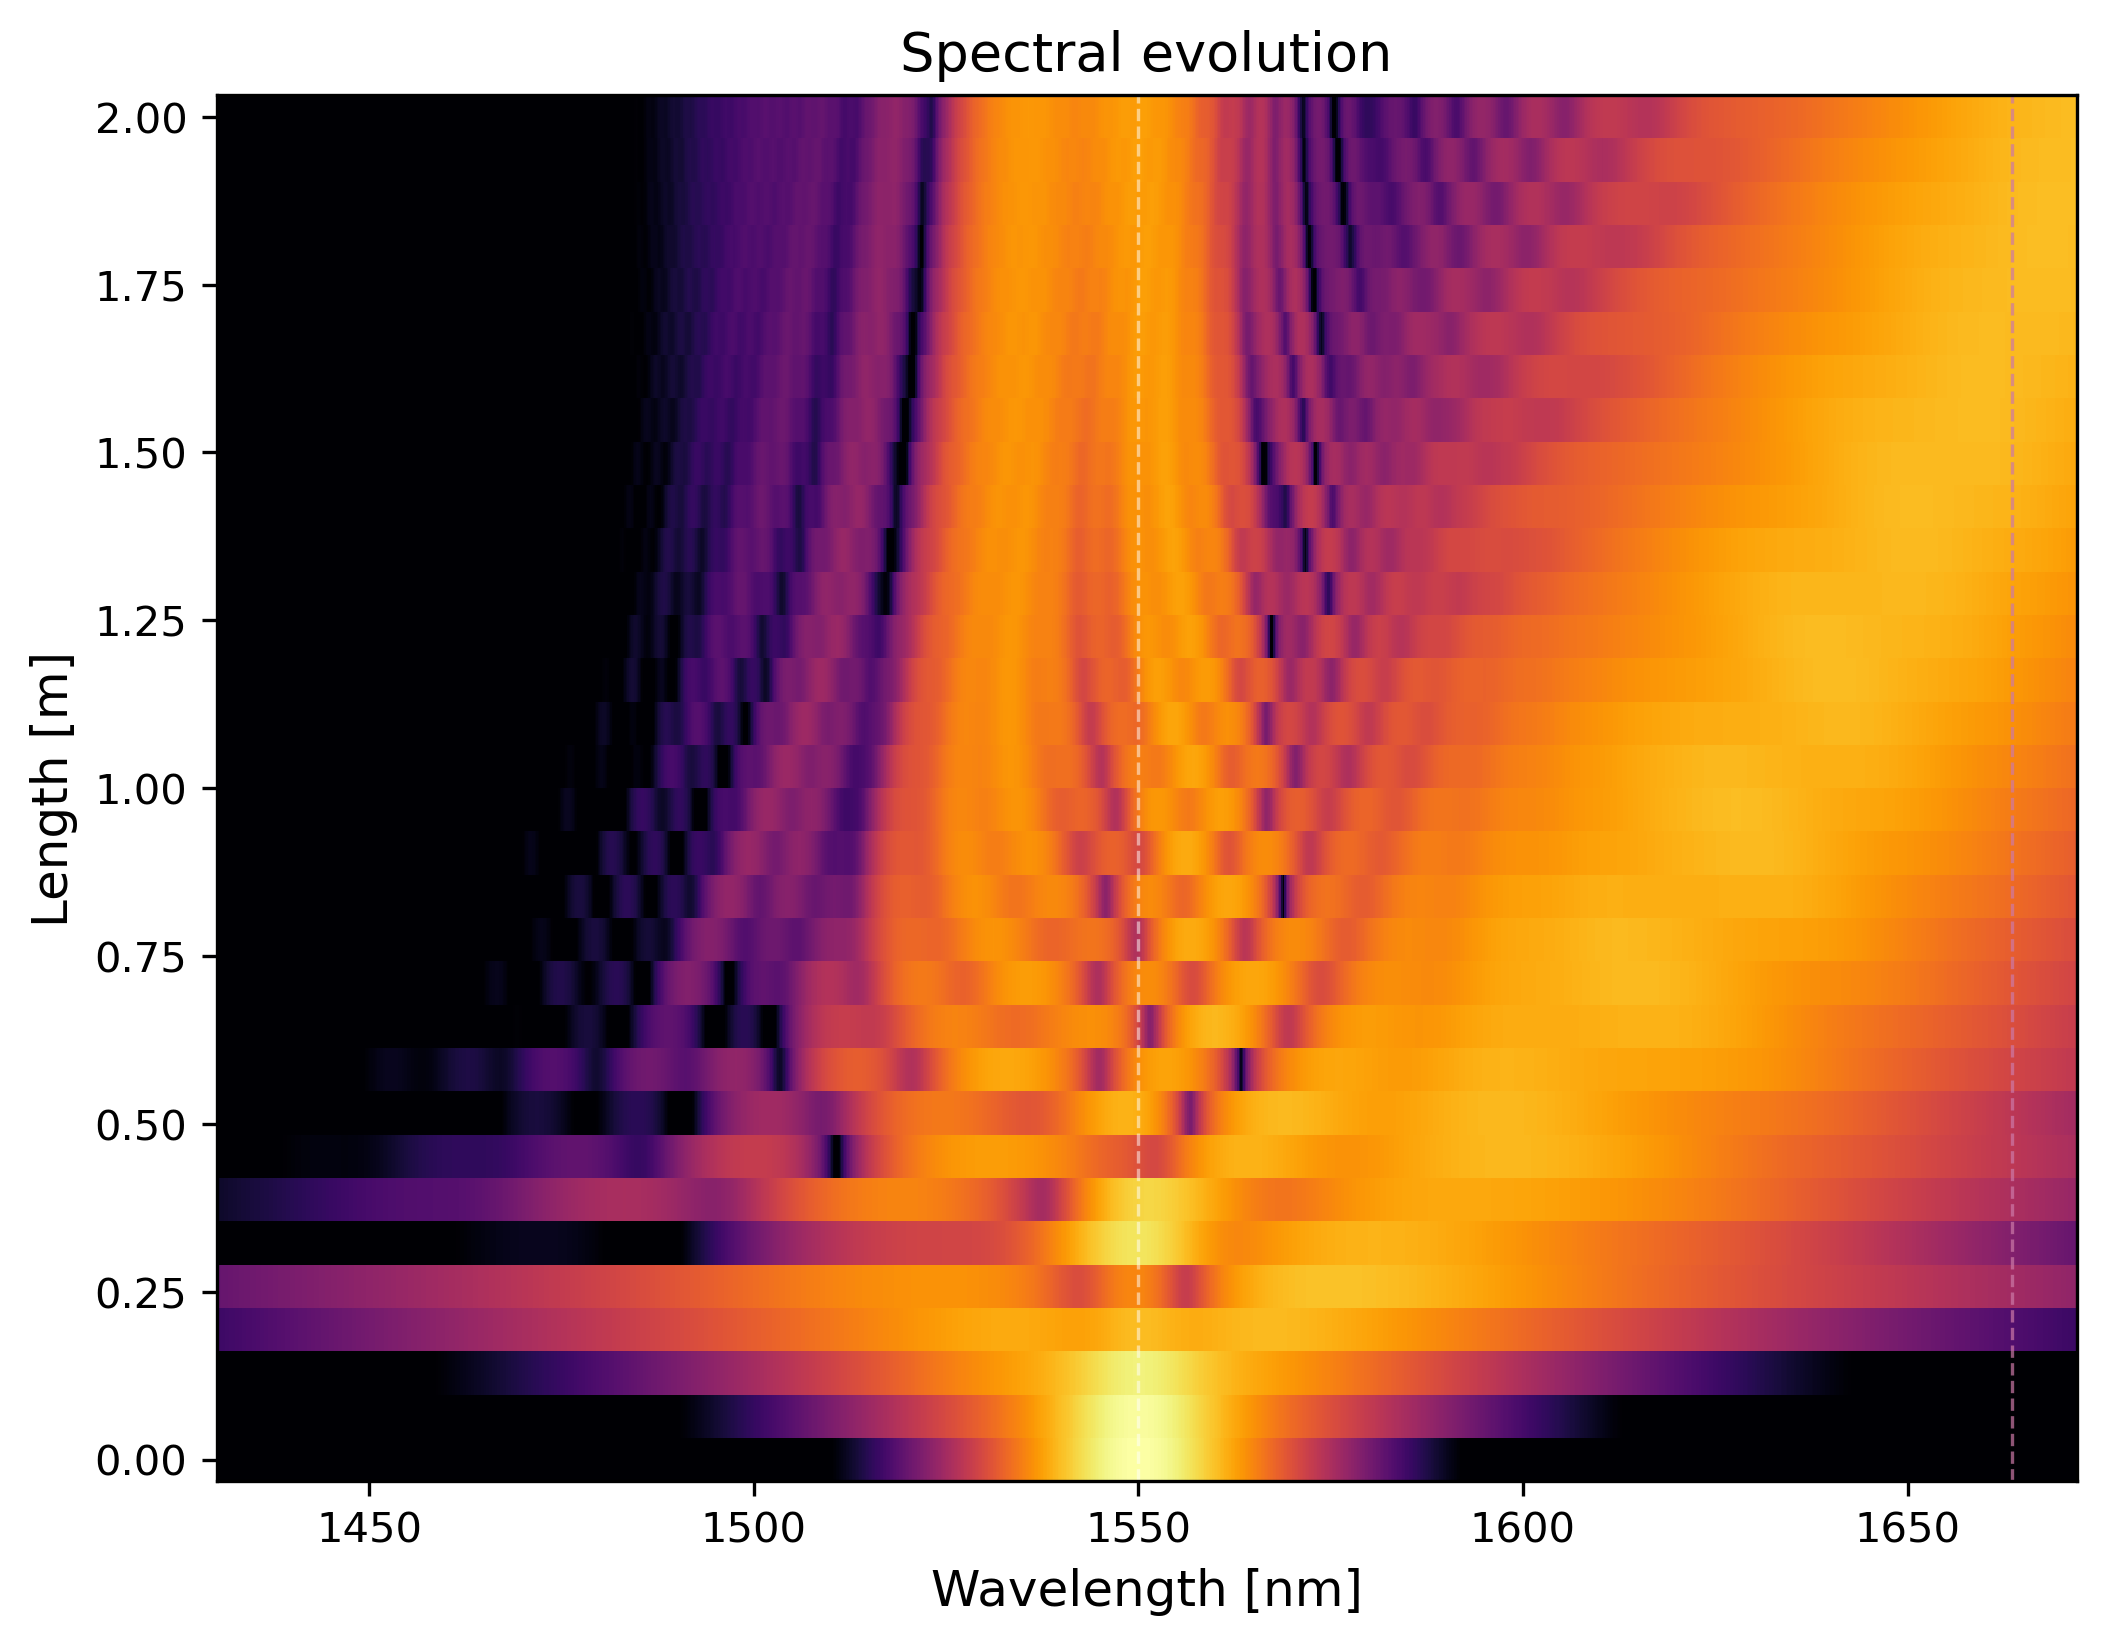
\includegraphics[height=0.31\textheight]{figures/control_no_optimization_evolution.png}
\caption{No-optimization control. The phase is flat, and the heat map shows
the unshaped spectral evolution. This is the reference behavior that the
optimized runs must beat.}
\end{figure}

\begin{figure}[p]
\centering
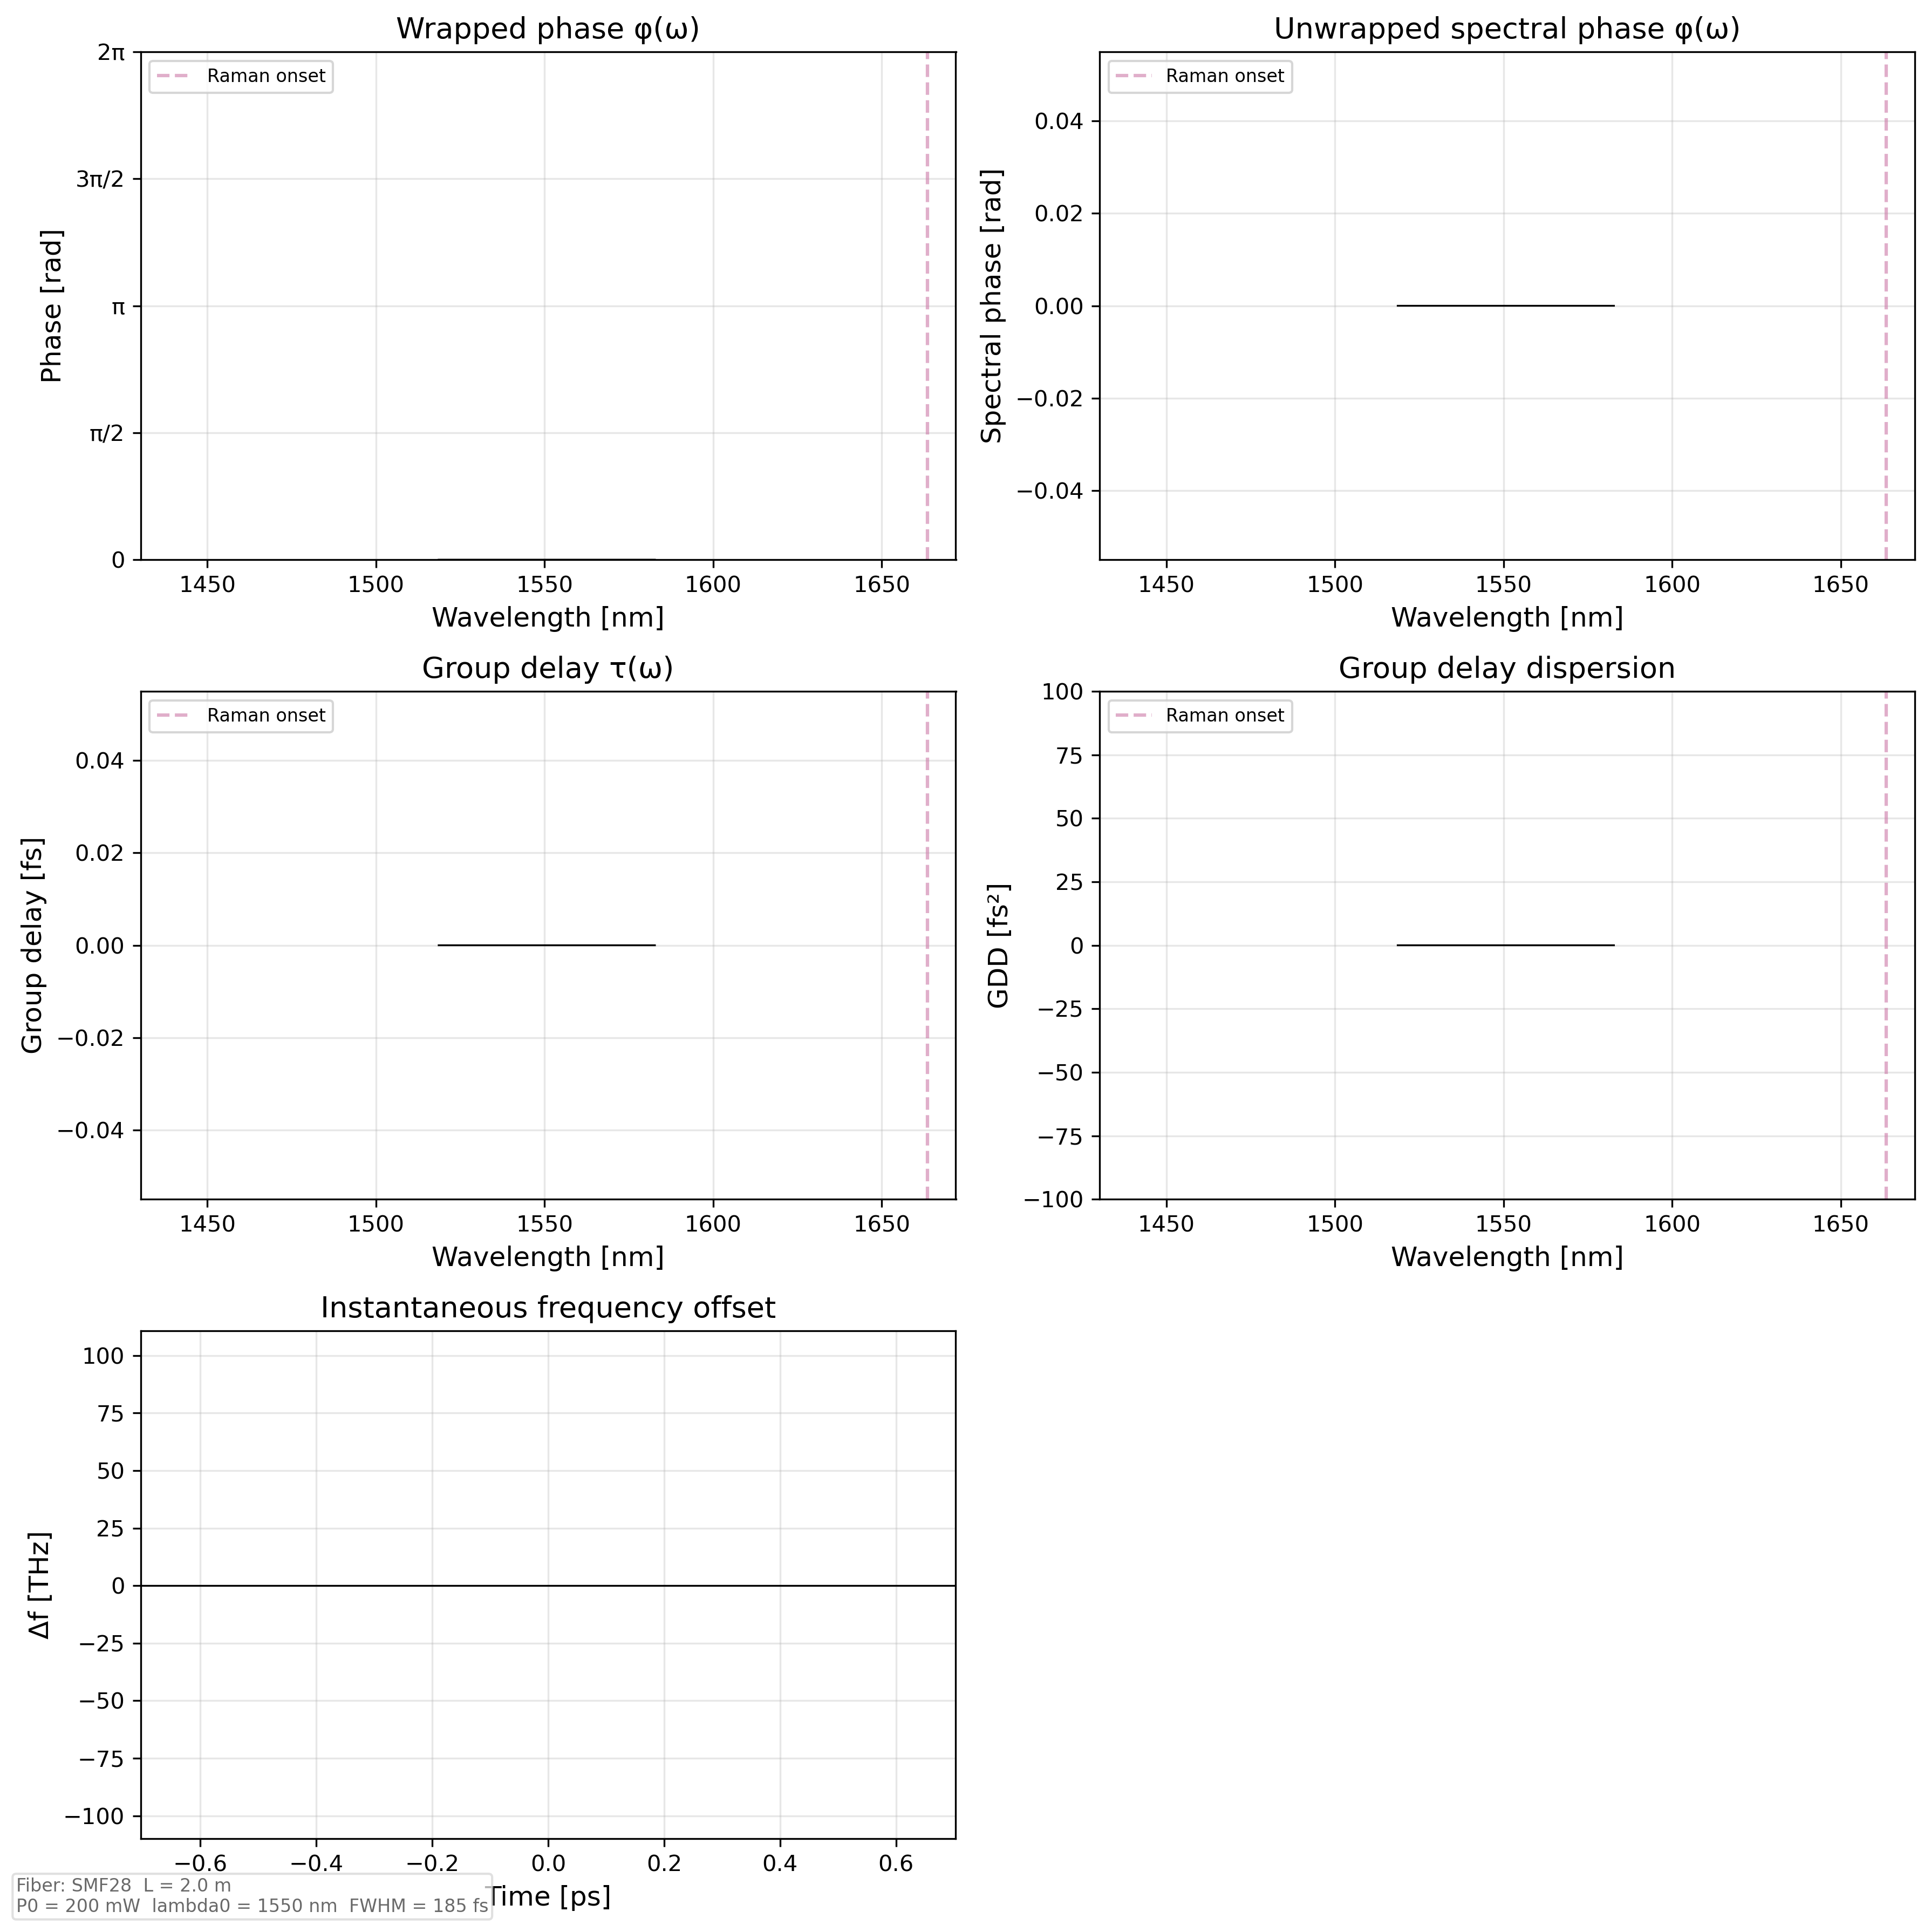
\includegraphics[height=0.48\textheight]{figures/cold_radius_collapse_phase_diagnostic.png}
\par\vspace{0.5em}
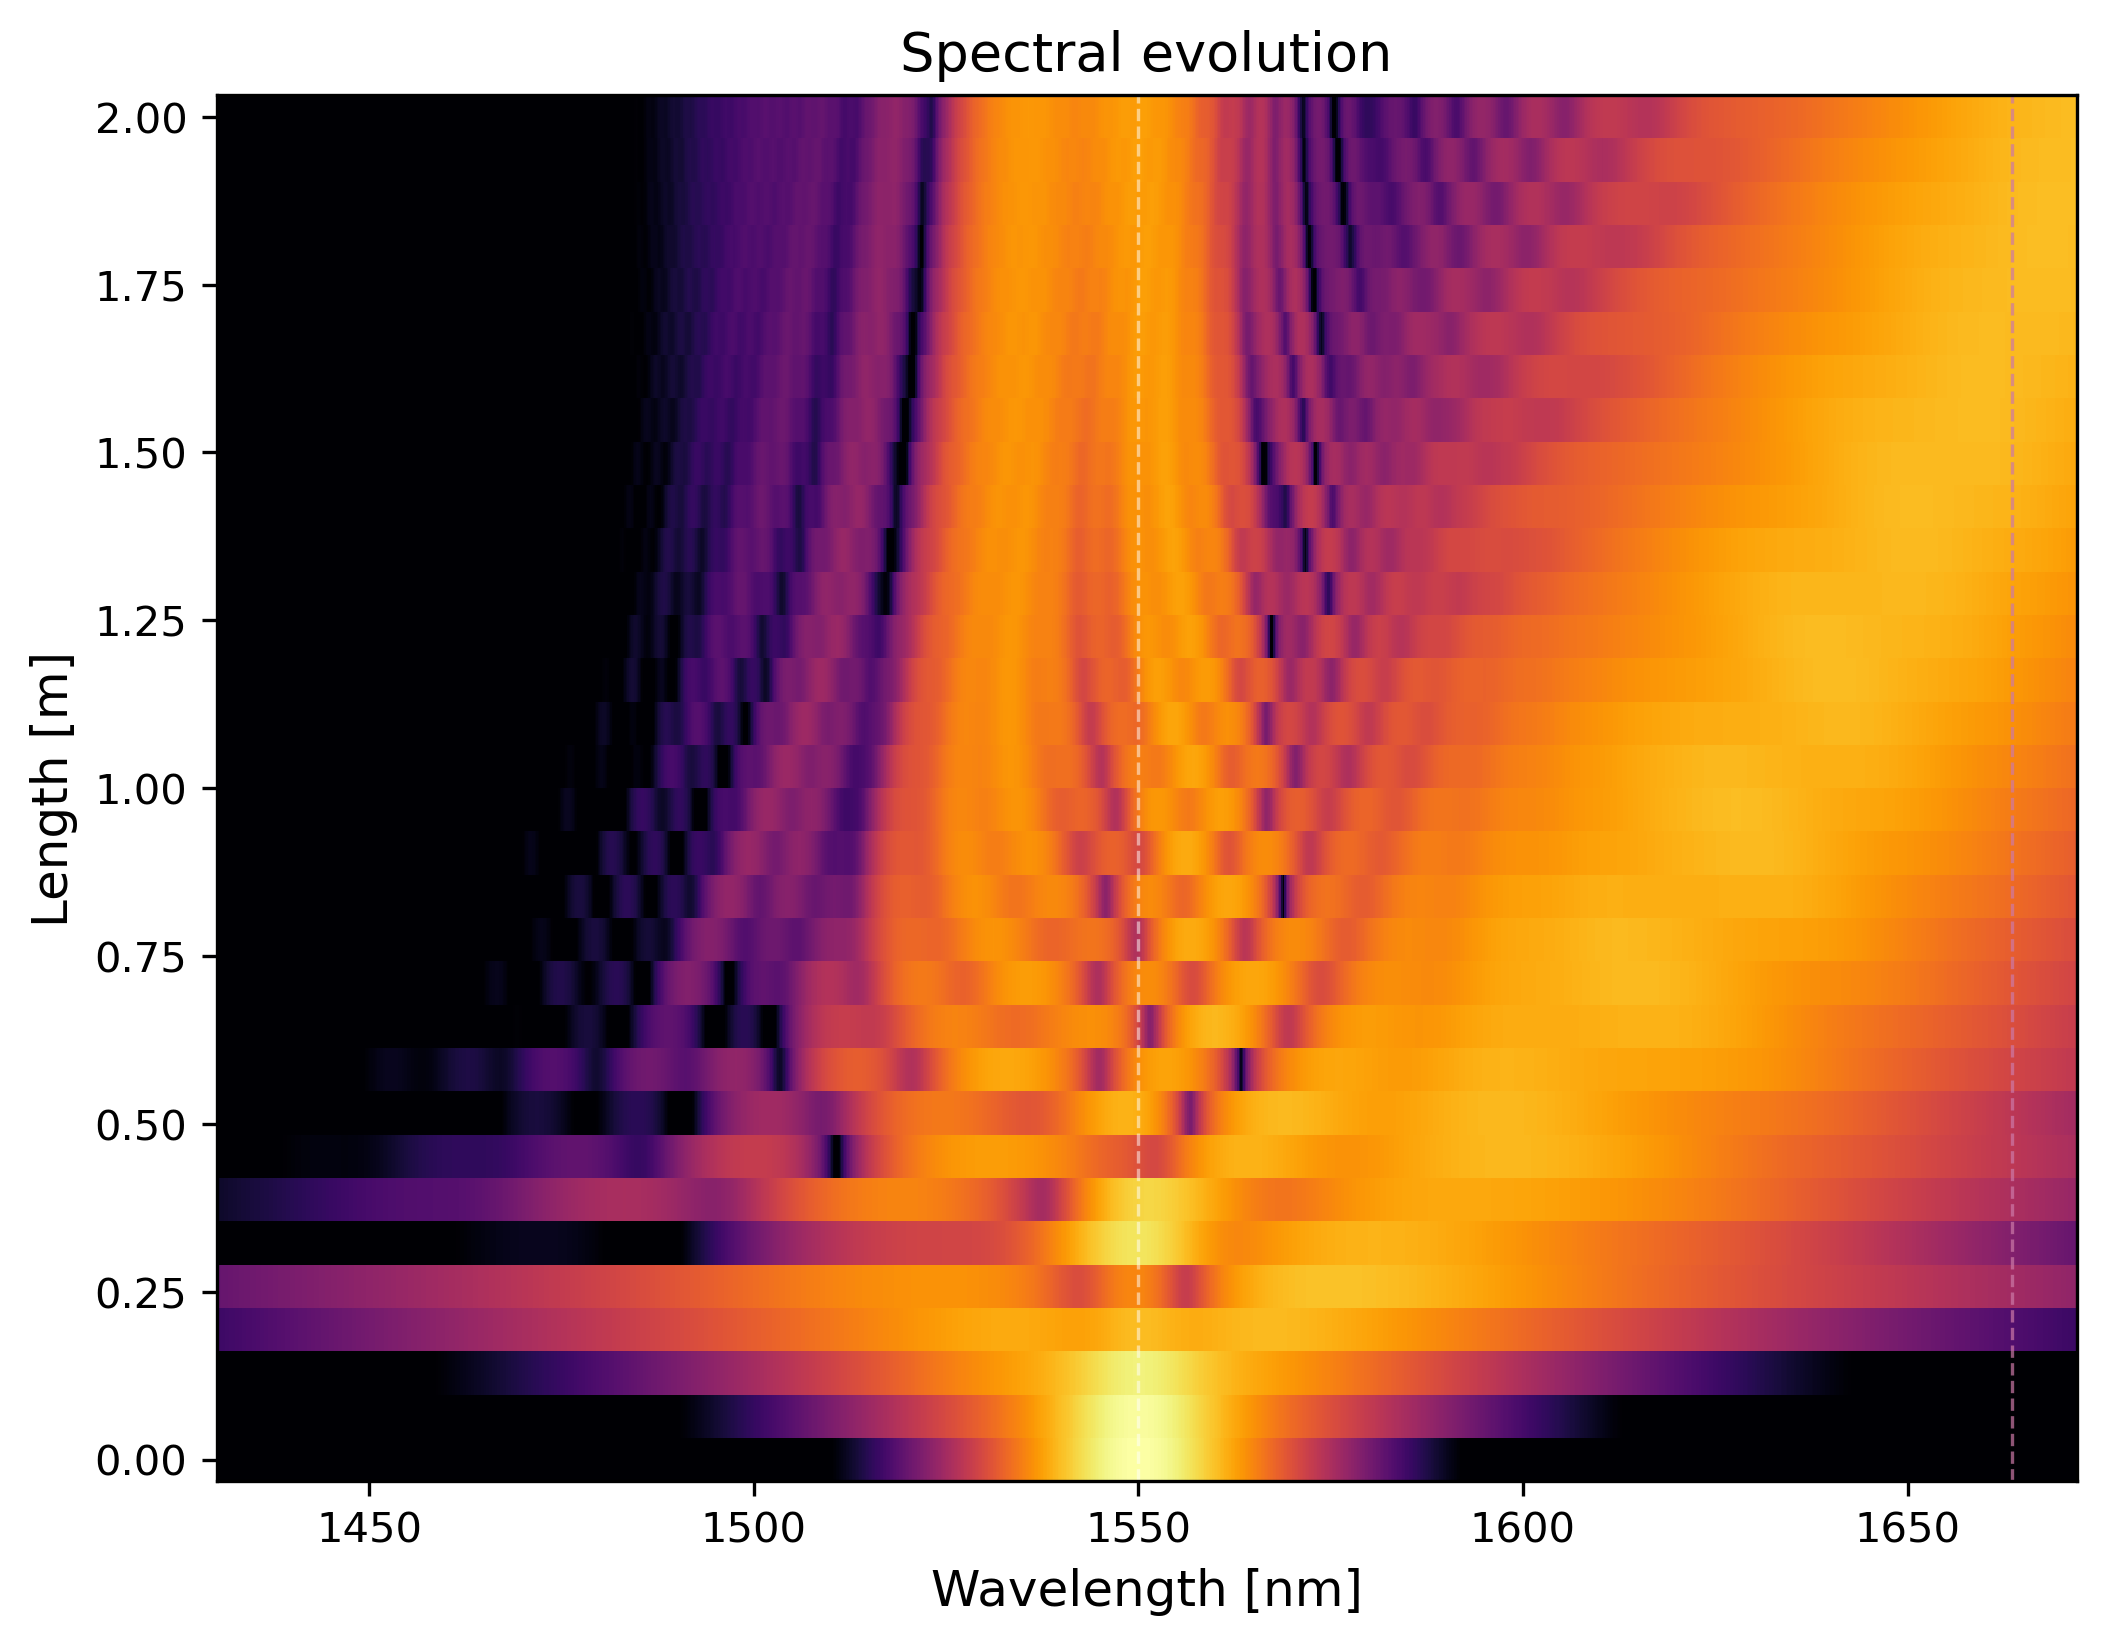
\includegraphics[height=0.31\textheight]{figures/cold_radius_collapse_evolution.png}
\caption{Cold-start trust-region collapse. Since no step was accepted, the
phase diagnostic remains essentially the same as the control, which visually
matches the numerical result that the objective did not improve.}
\end{figure}

\begin{figure}[p]
\centering
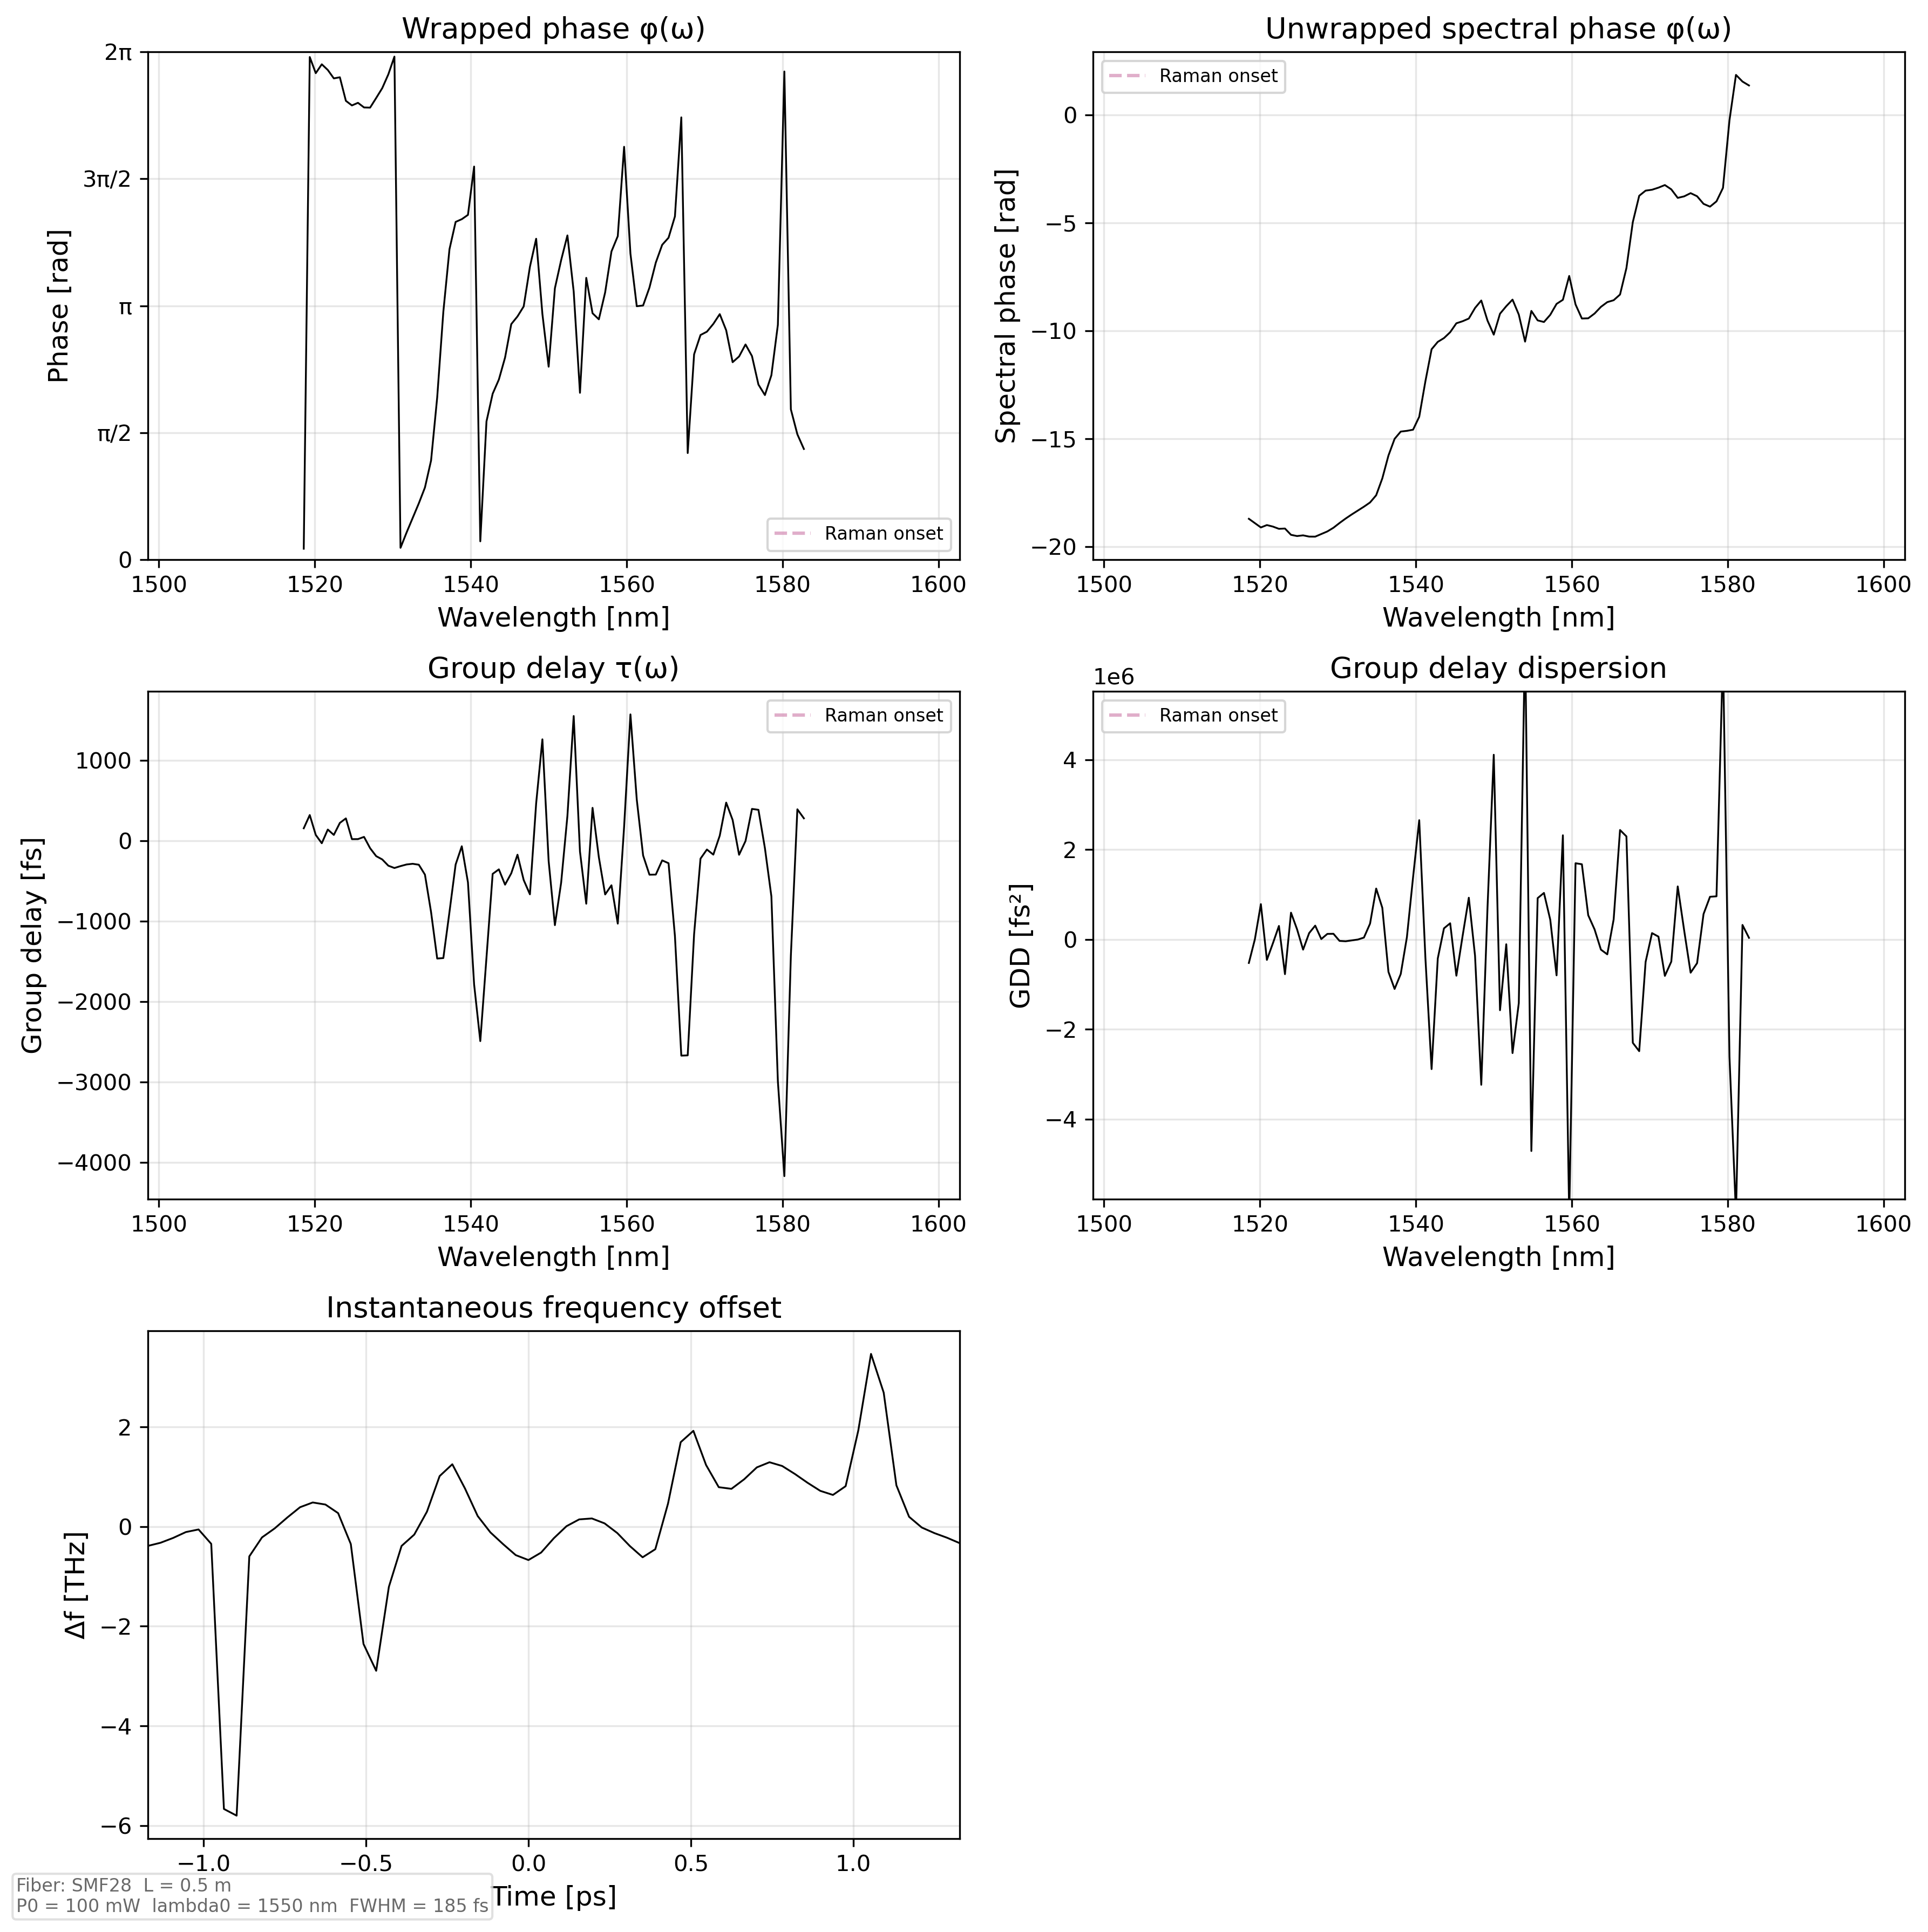
\includegraphics[height=0.48\textheight]{figures/continuation_seed_phase_diagnostic.png}
\par\vspace{0.5em}
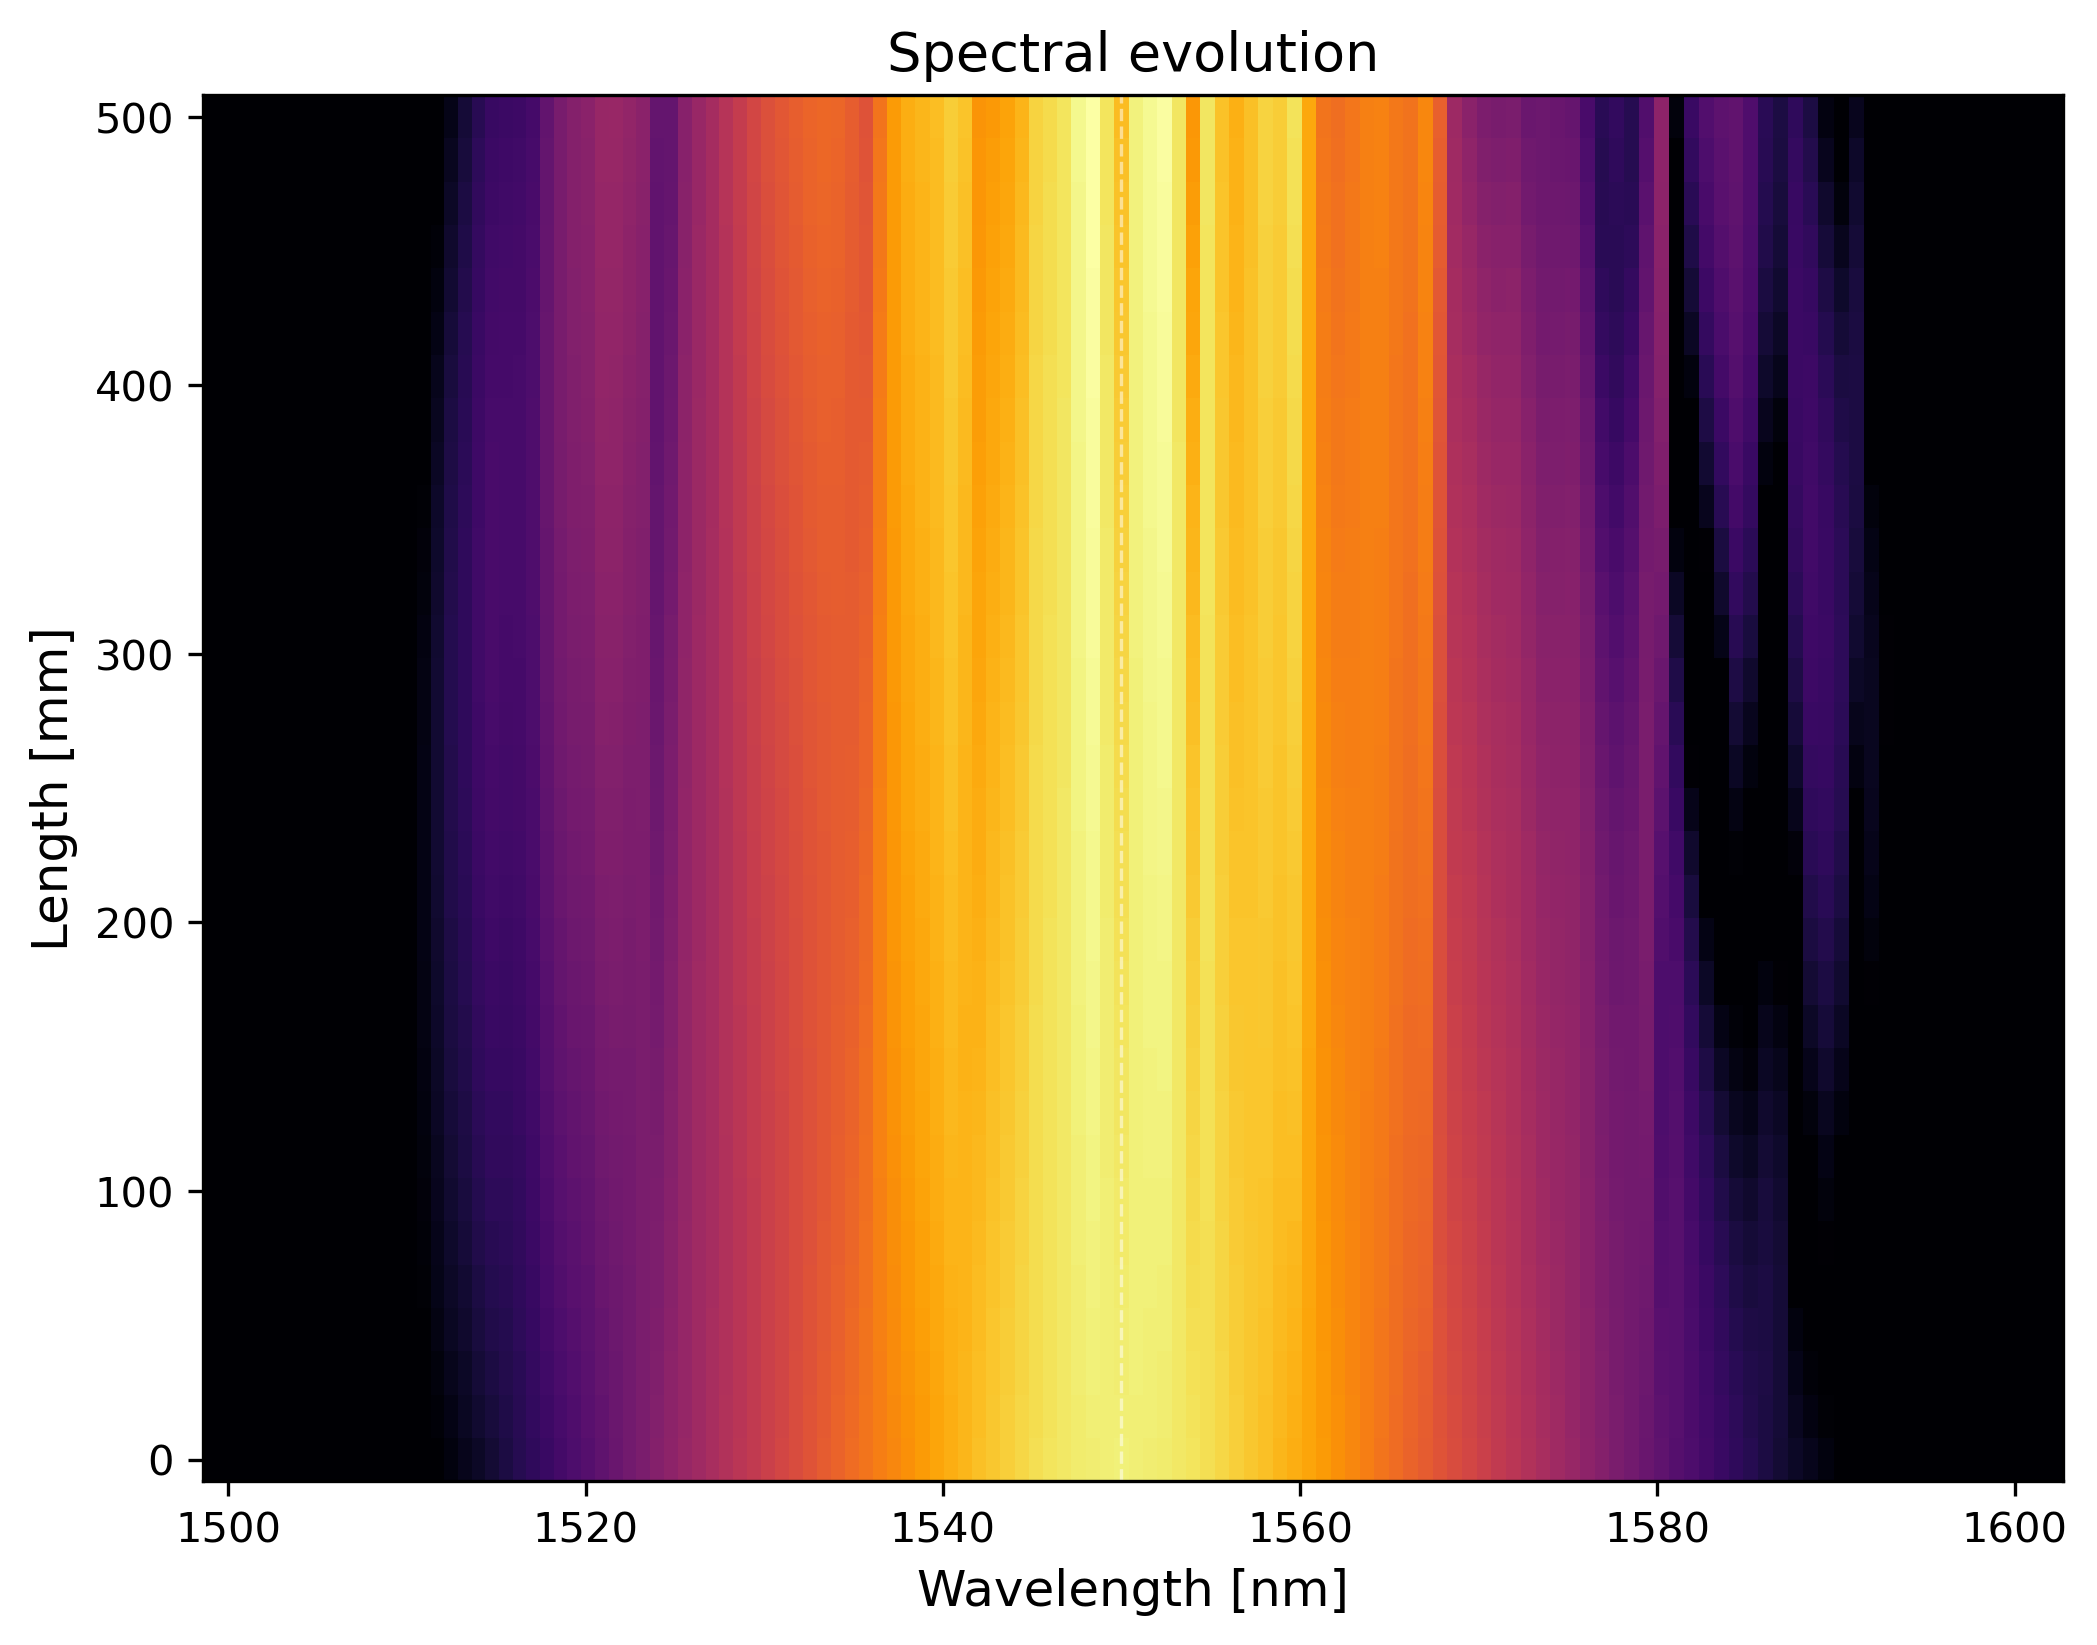
\includegraphics[height=0.31\textheight]{figures/continuation_seed_evolution.png}
\caption{Continuation seed from an easier fiber-length solve. This phase mask
is not produced by cold-start trust-region Newton; it is the kind of useful
starting point that continuation can supply.}
\end{figure}

\begin{figure}[p]
\centering
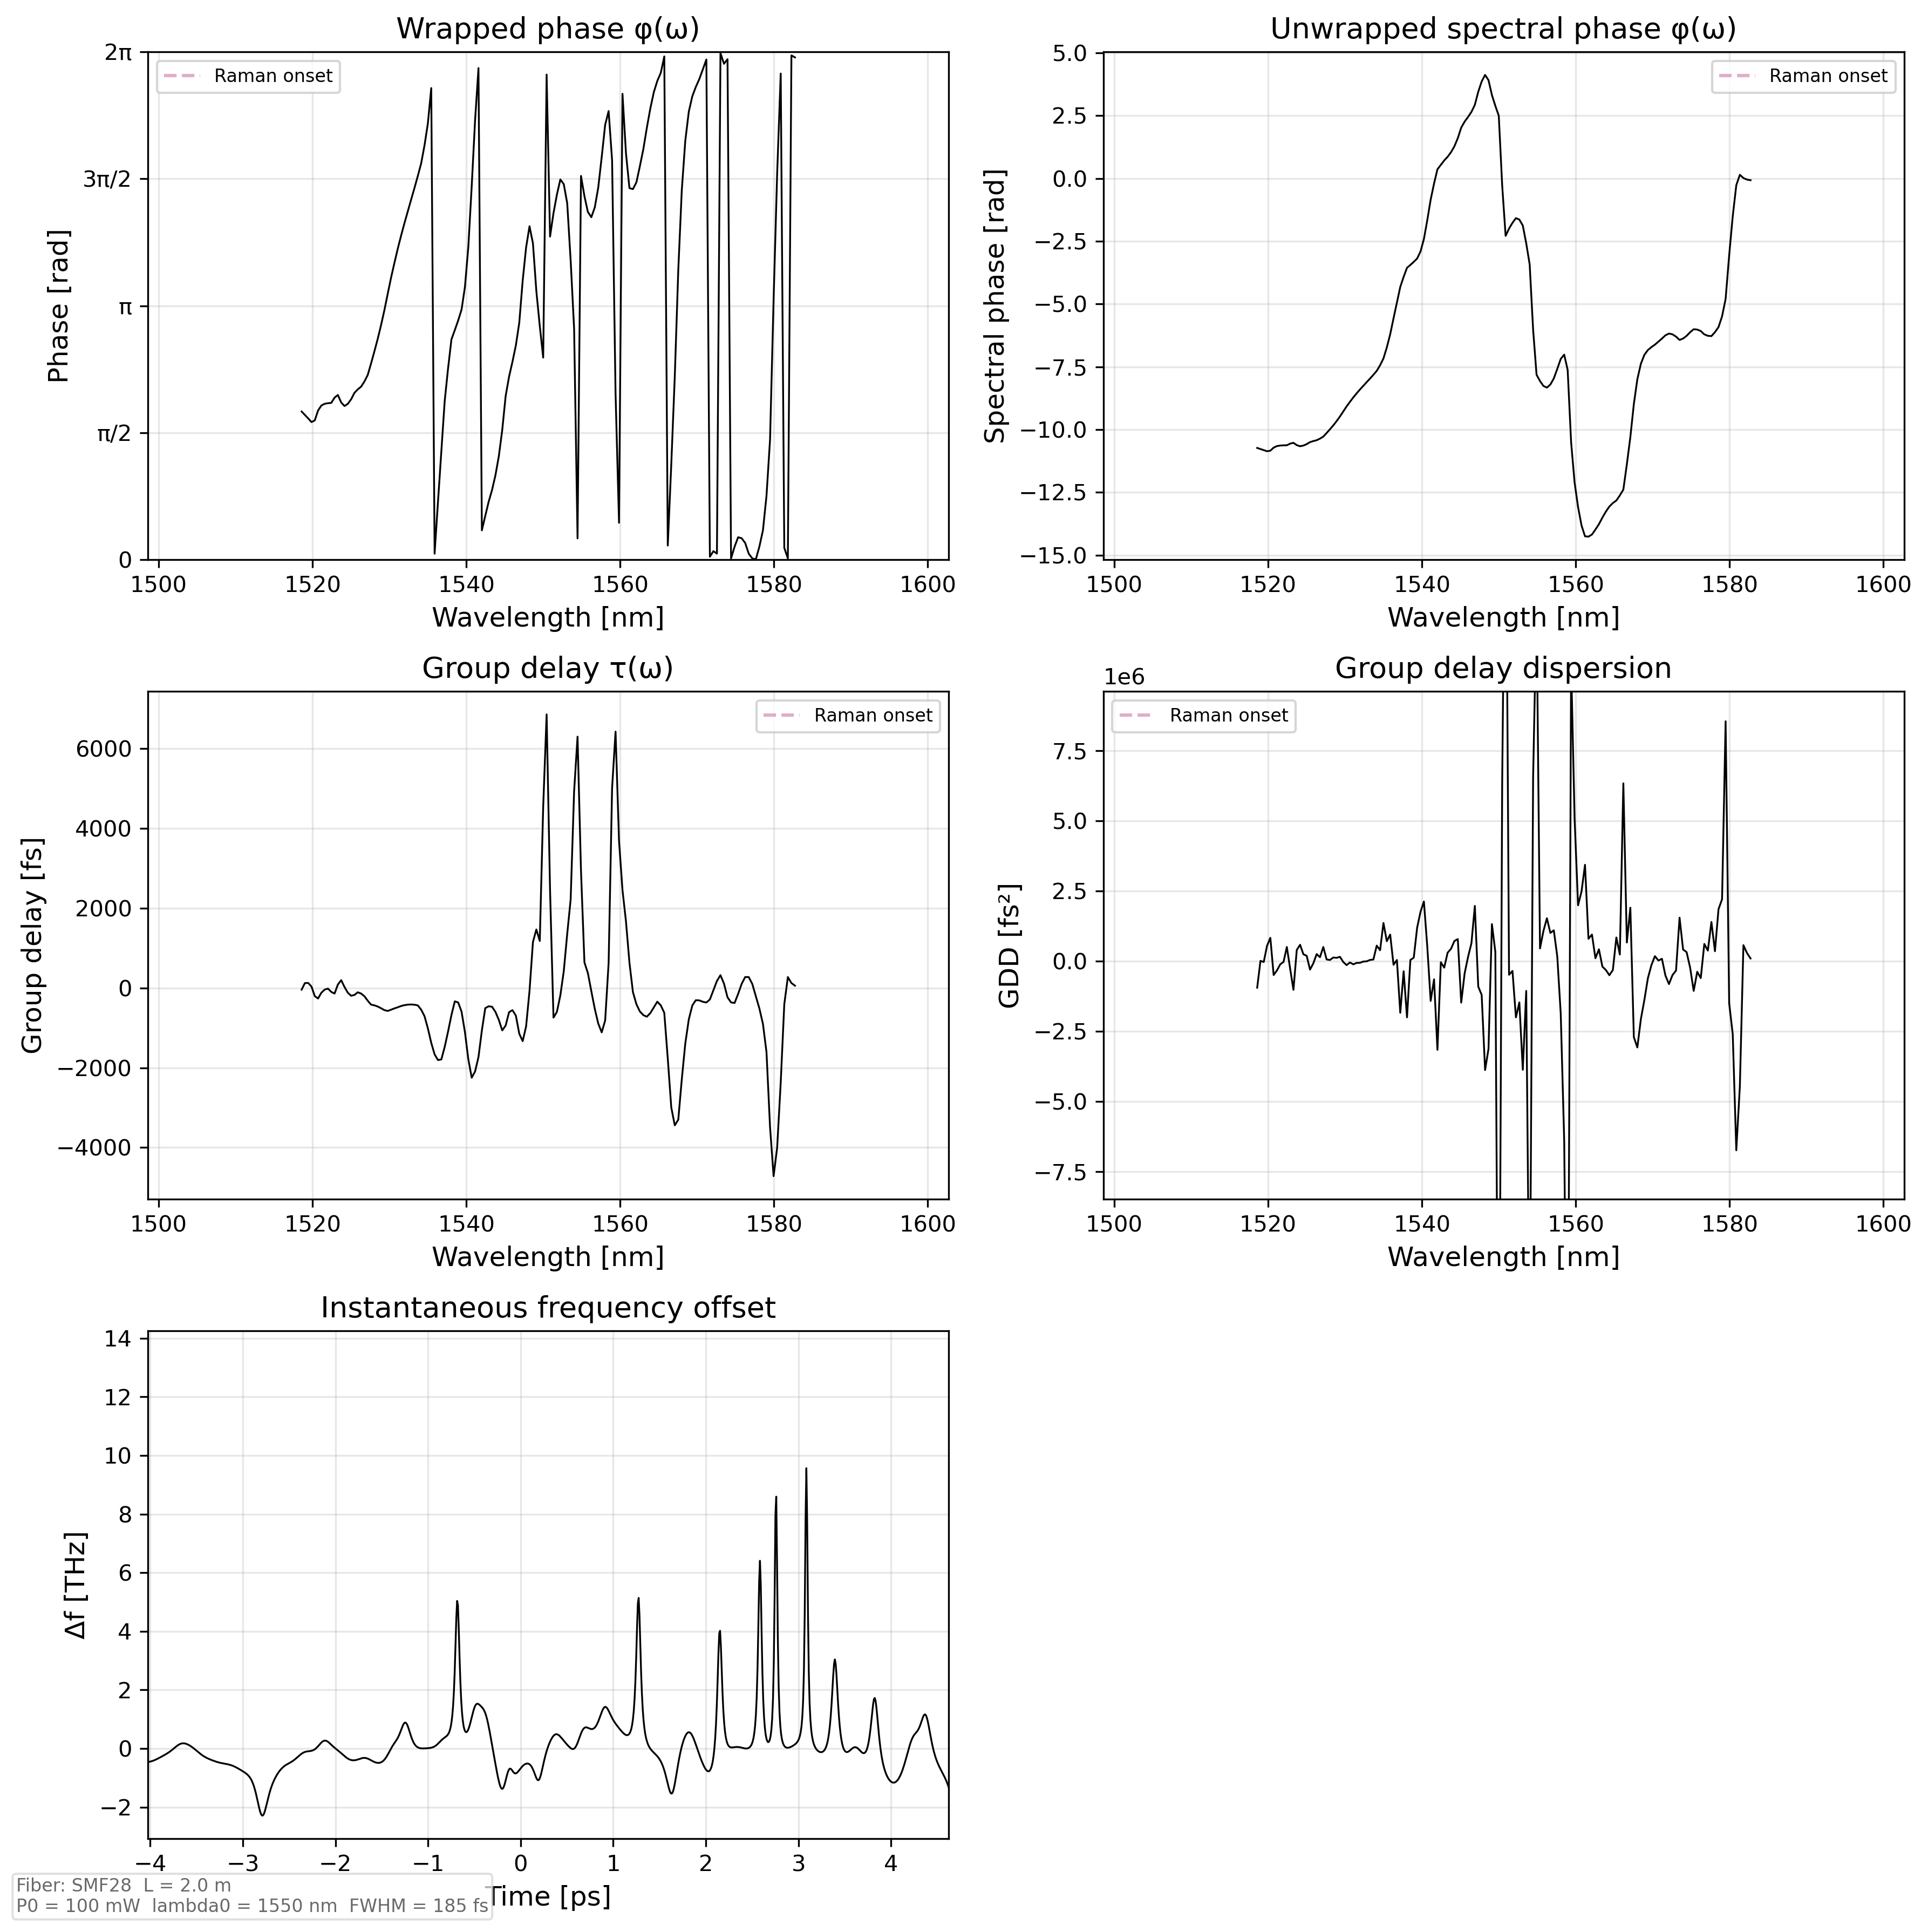
\includegraphics[height=0.48\textheight]{figures/ladder_no_preconditioner_phase_diagnostic.png}
\par\vspace{0.5em}
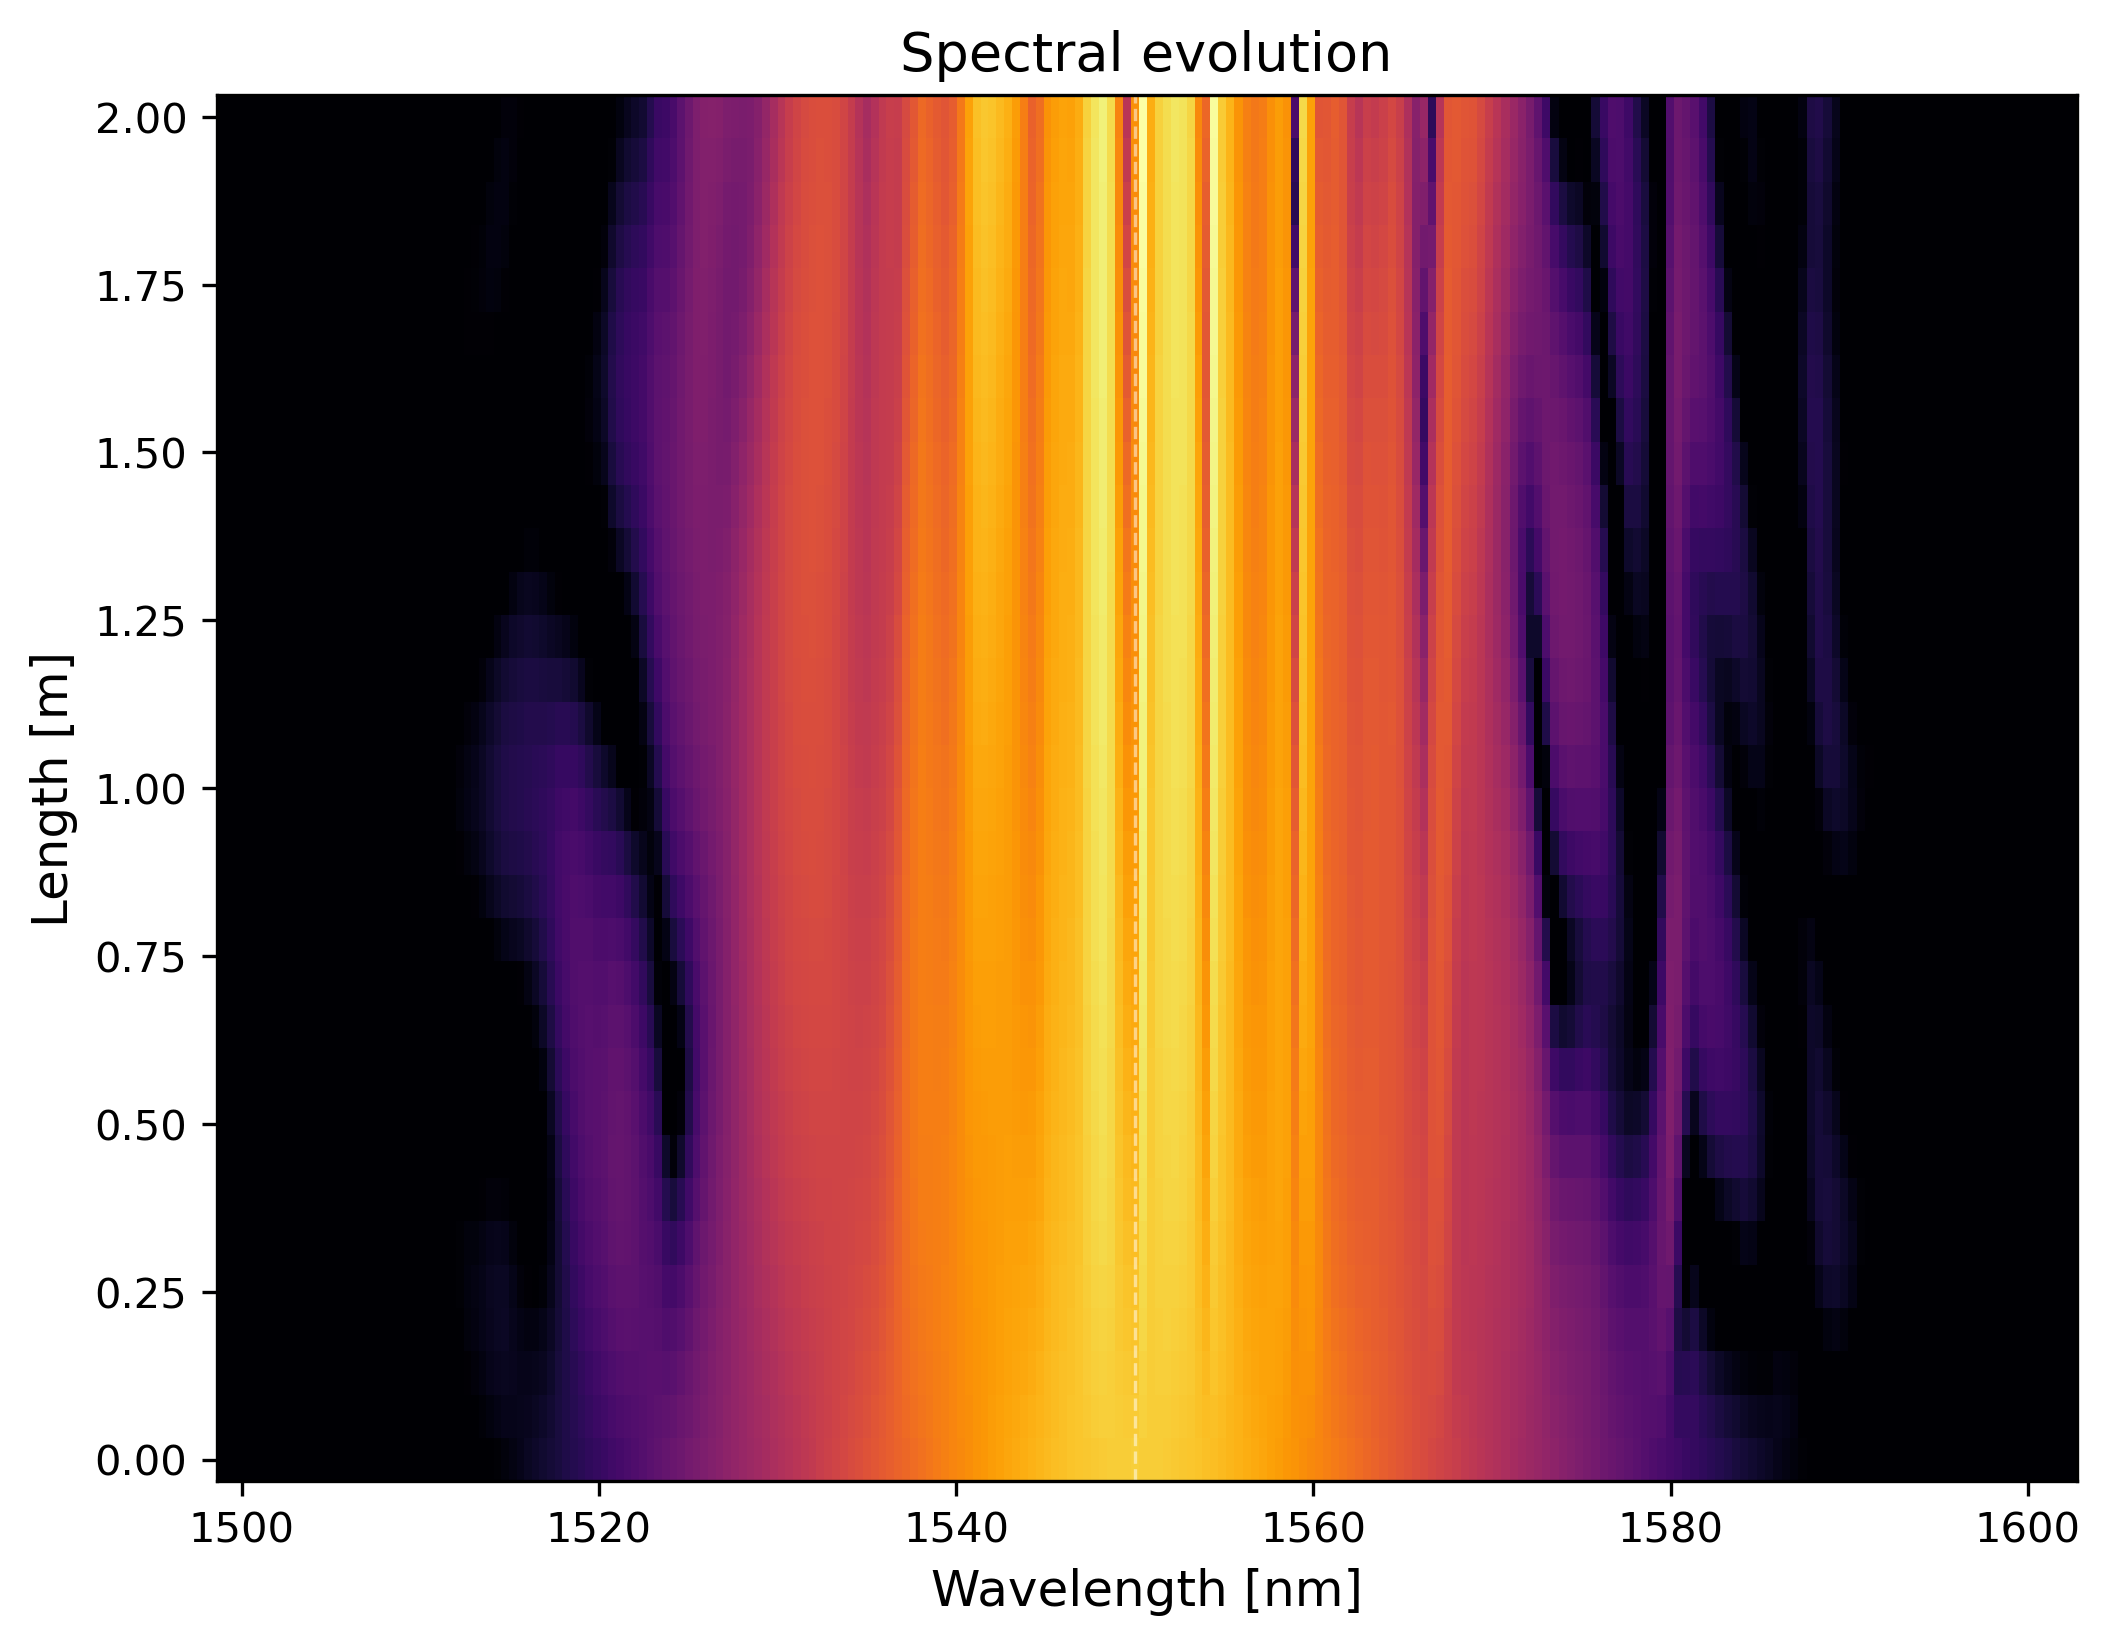
\includegraphics[height=0.31\textheight]{figures/ladder_no_preconditioner_evolution.png}
\caption{Continuation-assisted trust-region result without preconditioning on
the harder ladder rung. This is the honest baseline for the local
second-order comparison.}
\end{figure}

\begin{figure}[p]
\centering
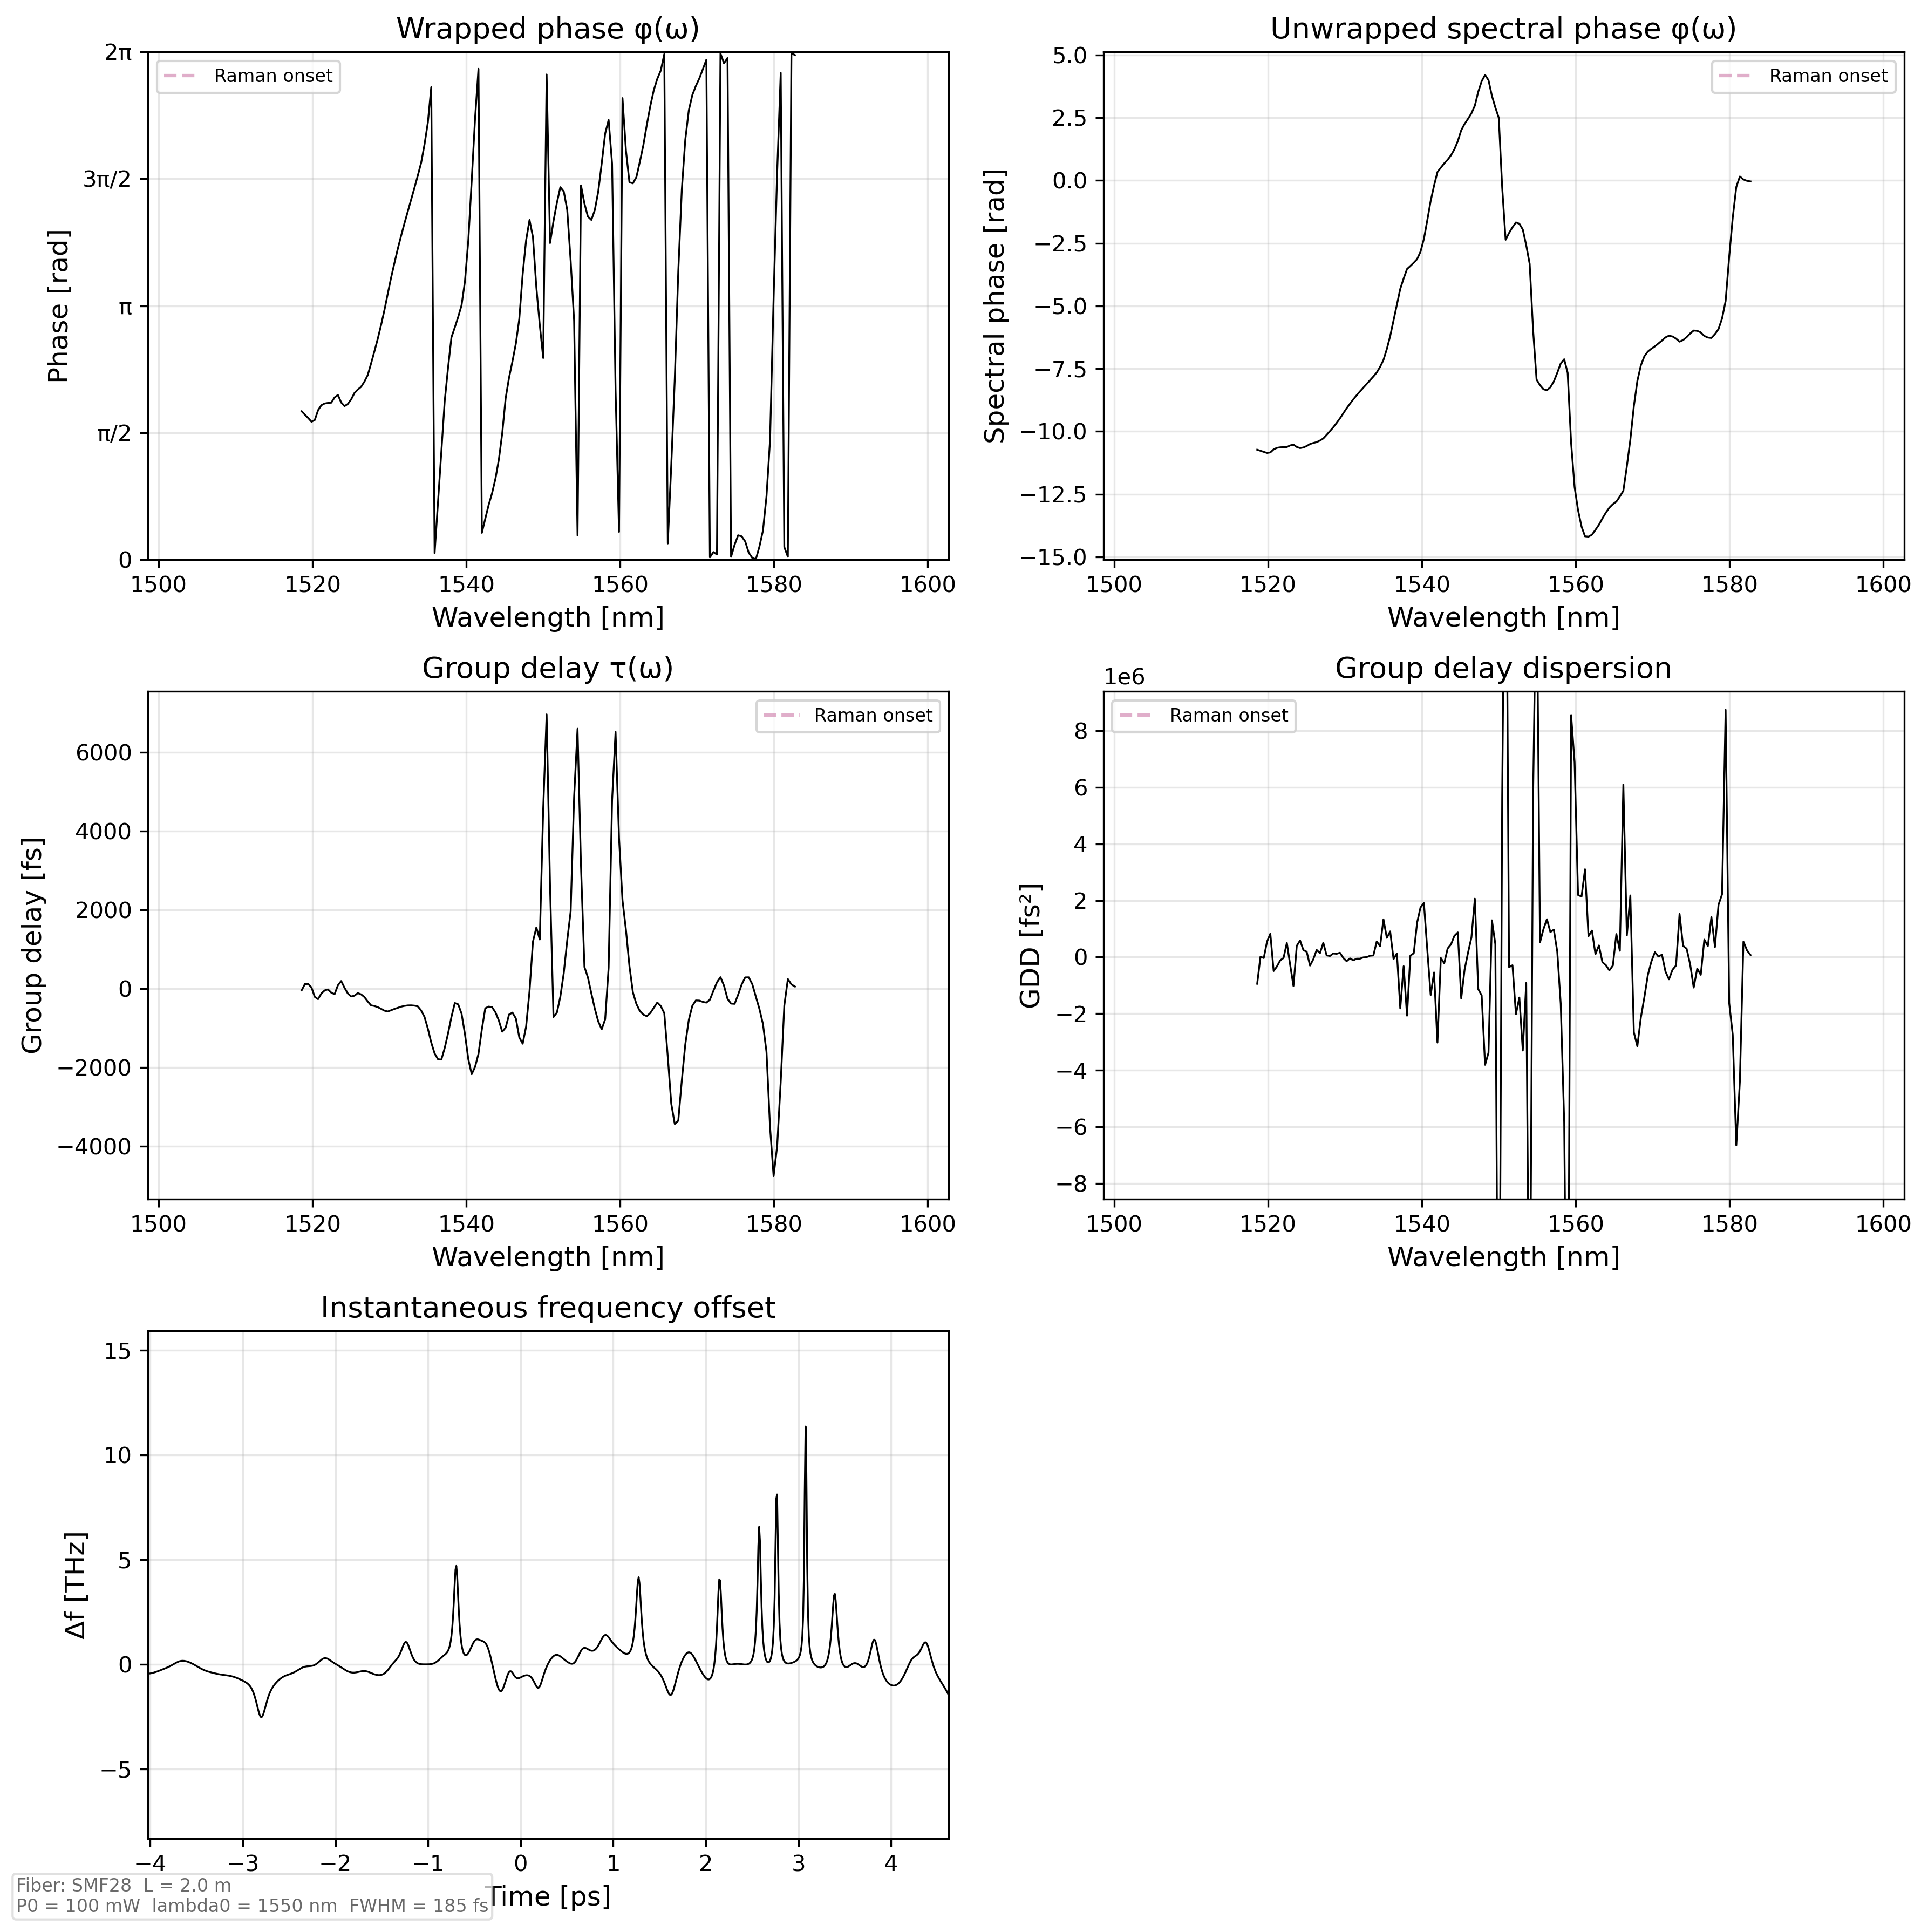
\includegraphics[height=0.48\textheight]{figures/ladder_dispersion_phase_diagnostic.png}
\par\vspace{0.5em}
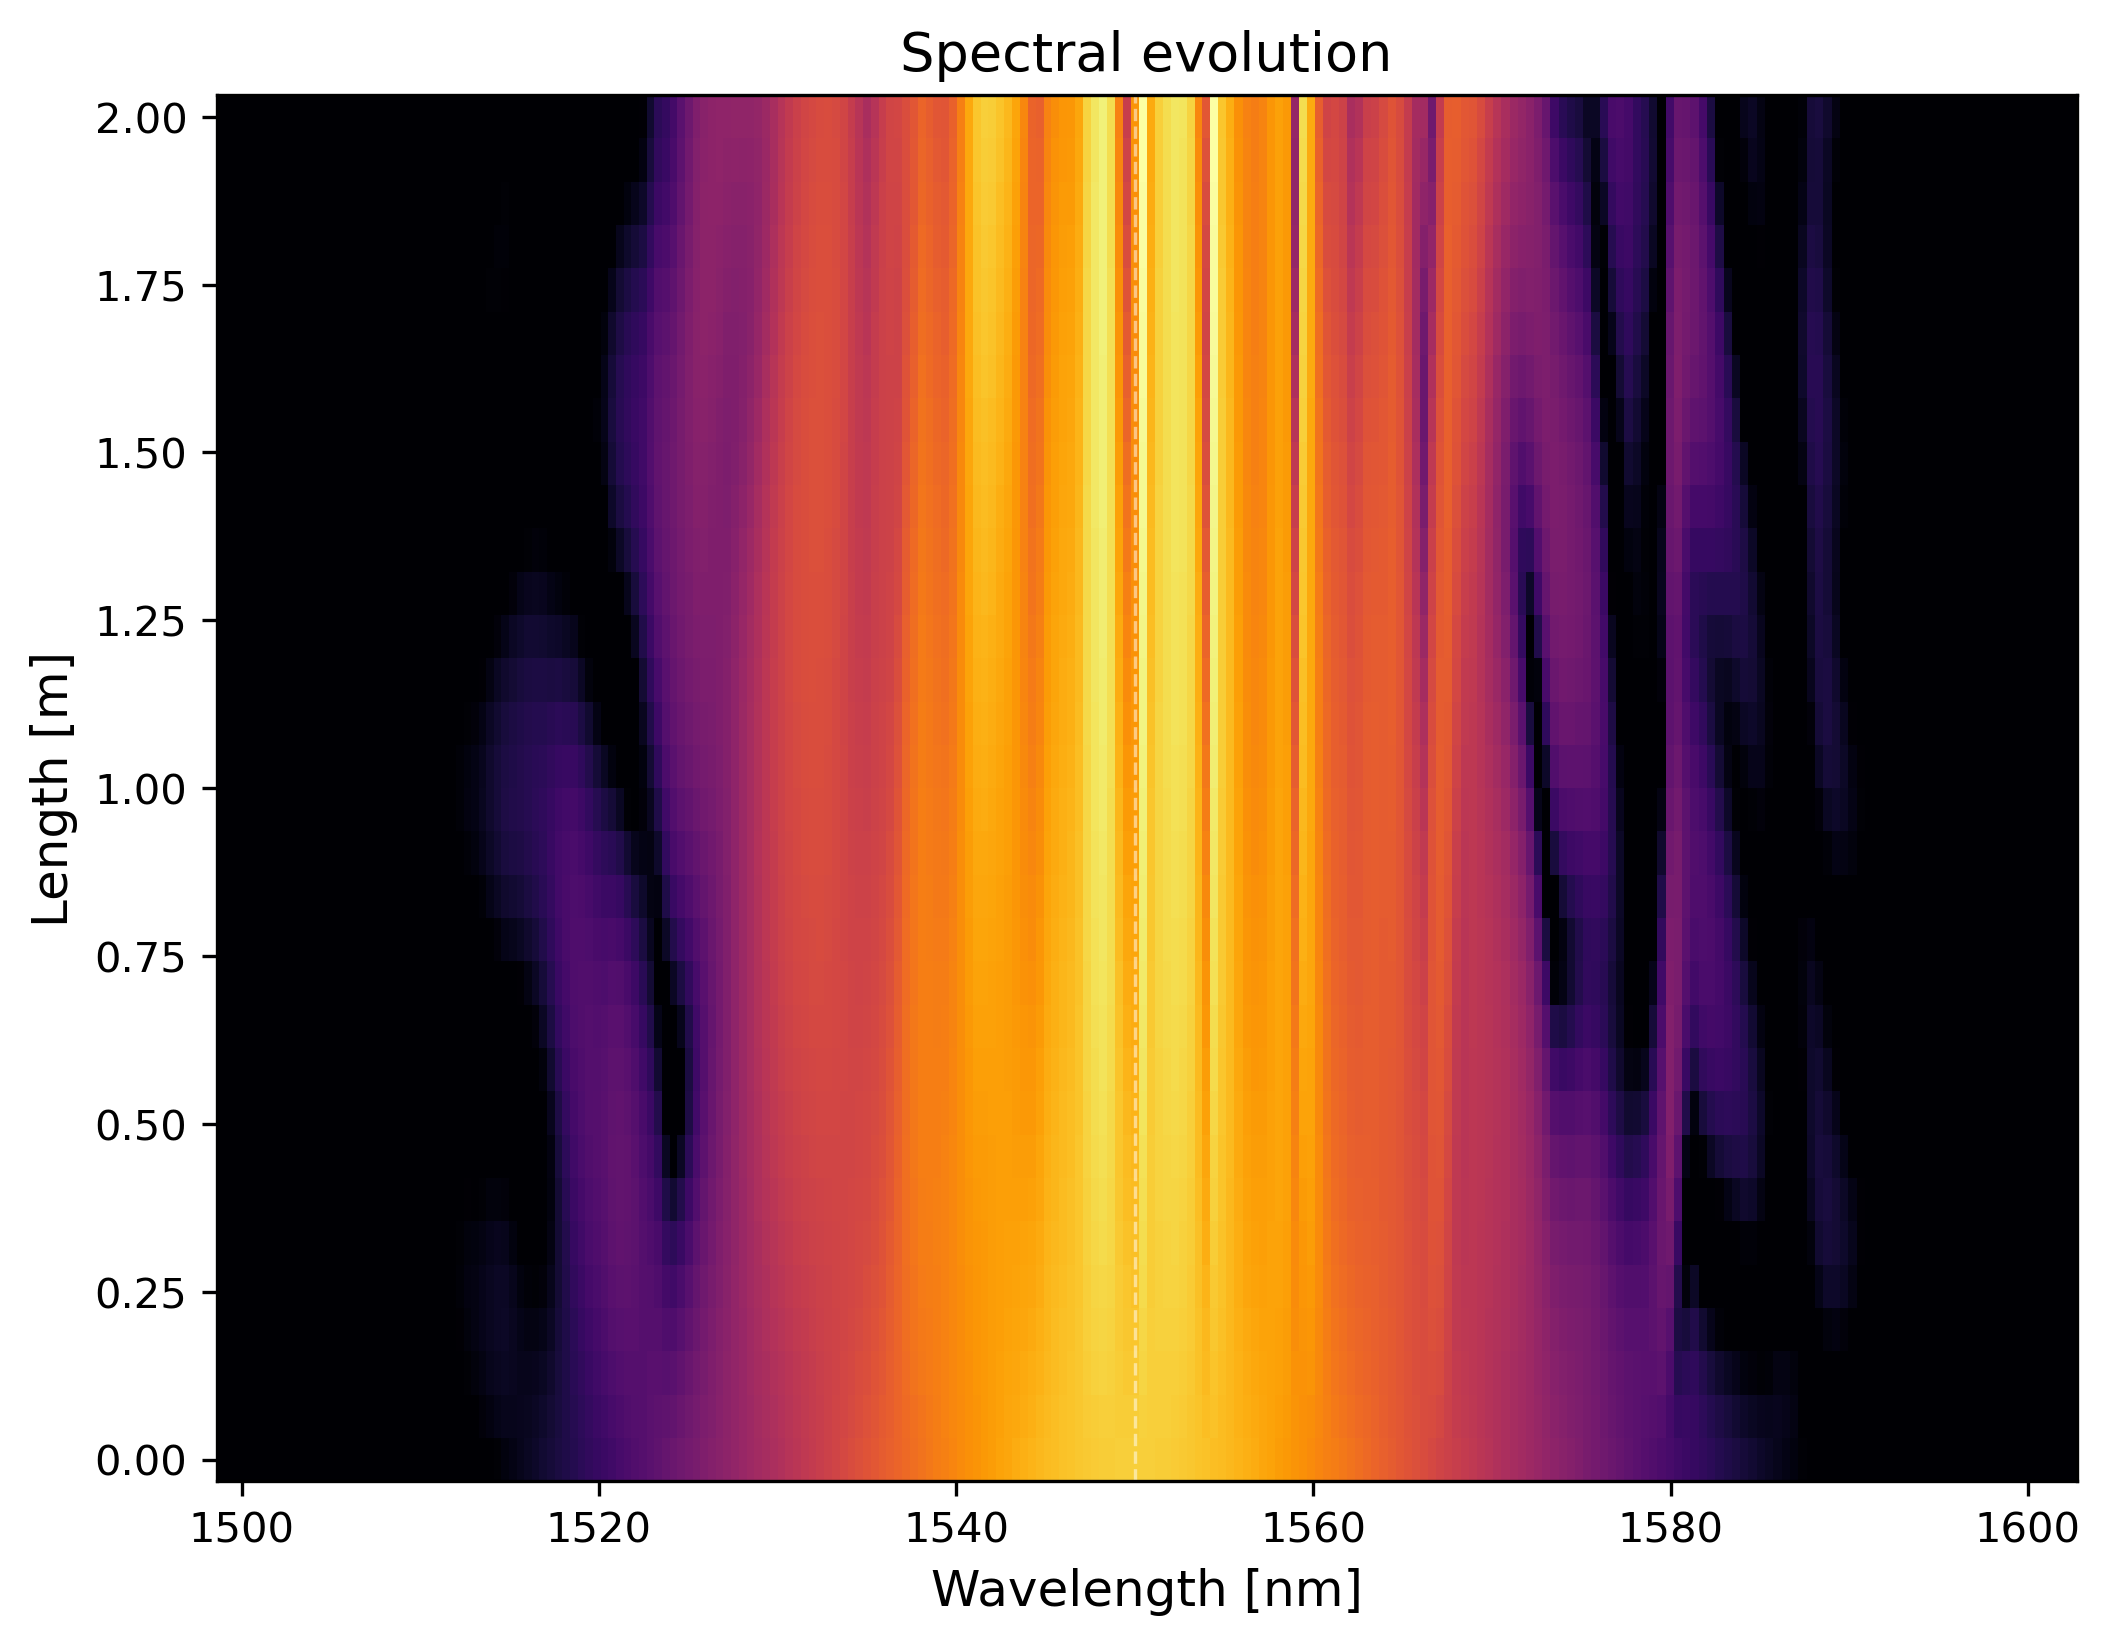
\includegraphics[height=0.31\textheight]{figures/ladder_dispersion_evolution.png}
\caption{Continuation-assisted trust-region result with dispersion
preconditioning on the same harder ladder rung. This was the clearest bounded
case where dispersion scaling improved the final objective and accepted-step
count.}
\end{figure}

\clearpage
\section{Continuation and Preconditioning Results}

\begin{figure}[H]
\centering
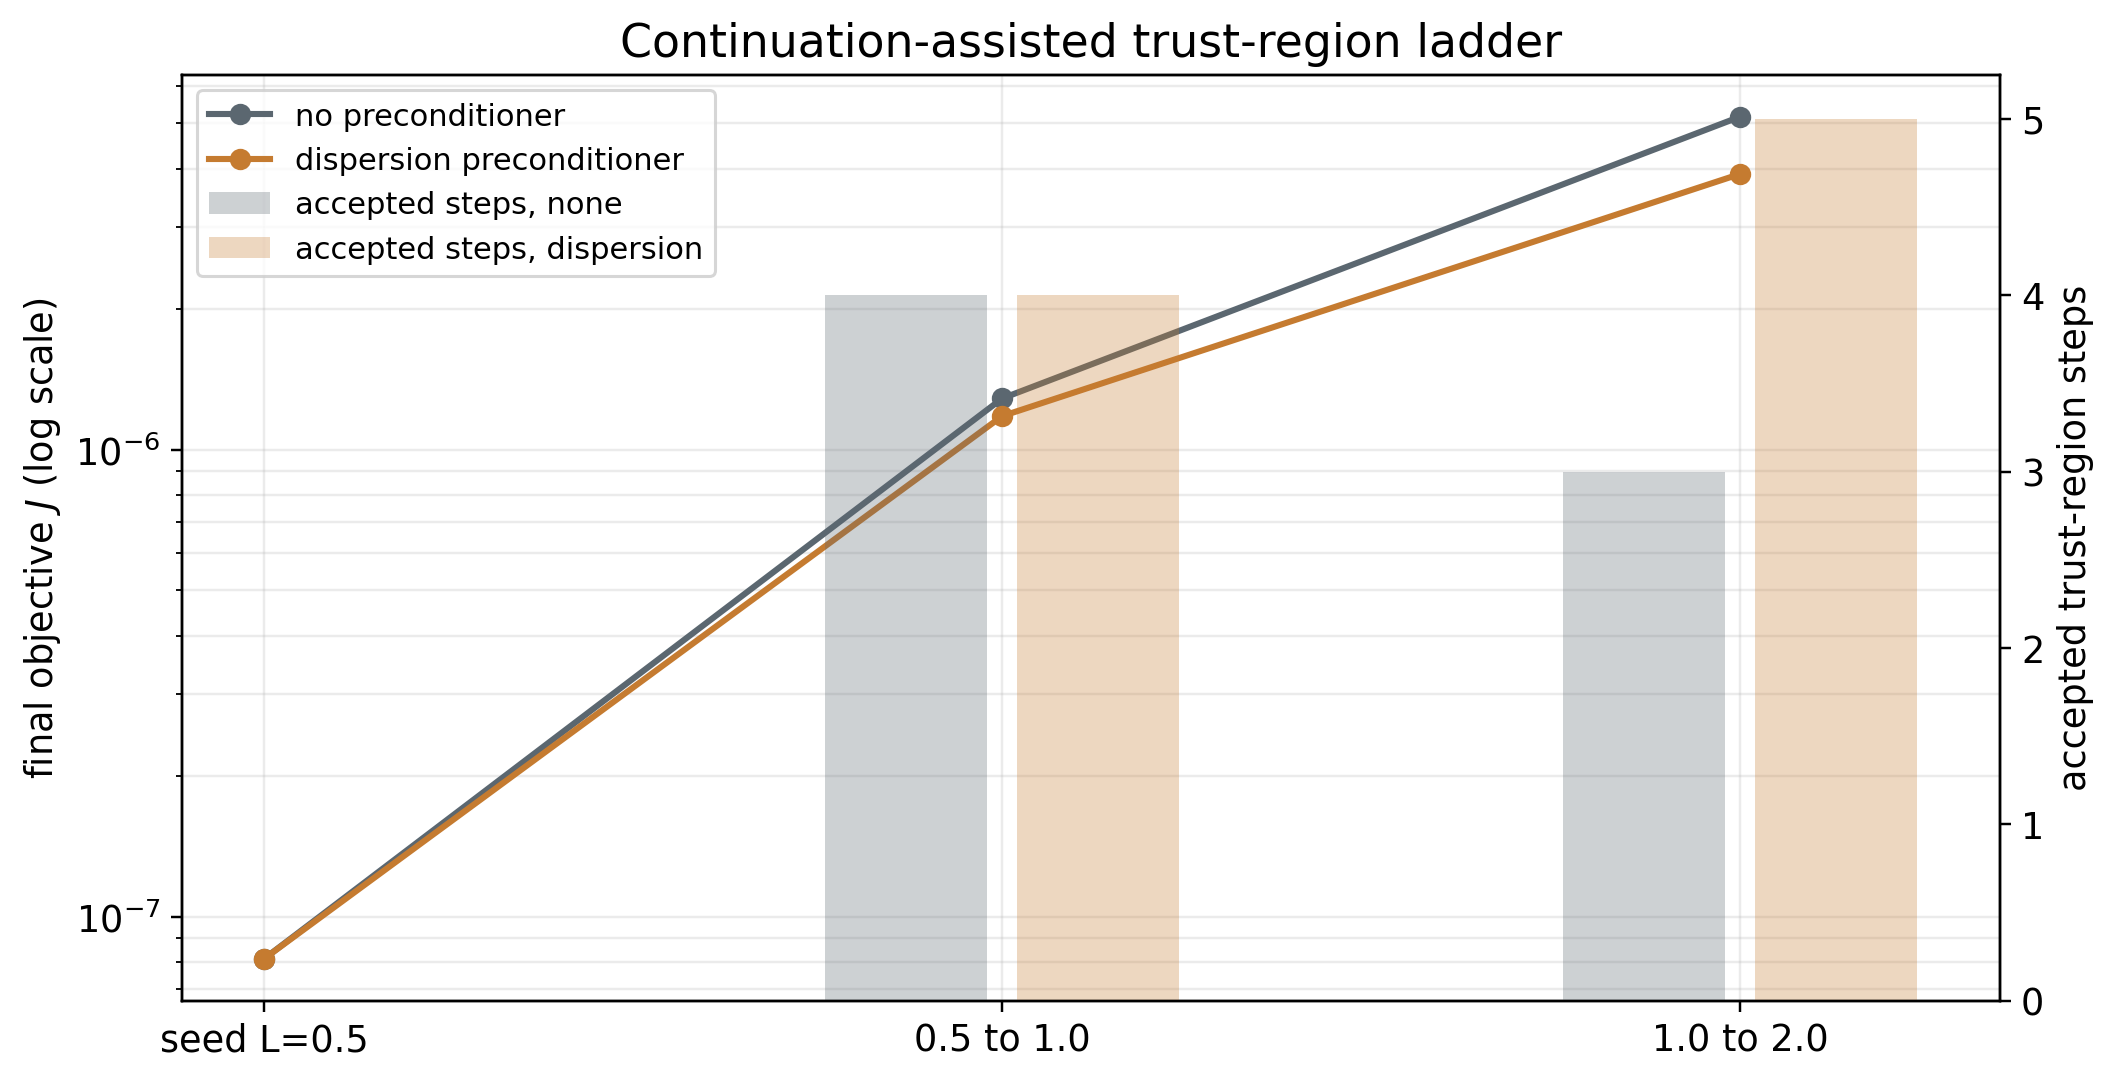
\includegraphics[width=0.88\linewidth]{figures/continuation_ladder_summary.png}
\caption{Short continuation ladder at fixed input power. Dispersion
preconditioning was modestly better than no preconditioner on the harder rung,
but only after continuation supplied a useful starting point.}
\end{figure}

\begin{center}
\scriptsize
\begin{tabular}{p{0.24\linewidth}p{0.20\linewidth}p{0.15\linewidth}p{0.12\linewidth}p{0.15\linewidth}}
\toprule
\textbf{Step} & \textbf{method} & \textbf{final \(J\)} & \textbf{accepted} & \textbf{exit} \\
\midrule
Seed \(L=0.5\,\mathrm{m}\) & L-BFGS & \(8.14\times10^{-8}\) & -- & converged \\
\(0.5\rightarrow1.0\,\mathrm{m}\) & no precond. & \(1.29\times10^{-6}\) & 4 & 1st-order saddle \\
\(0.5\rightarrow1.0\,\mathrm{m}\) & dispersion & \(1.18\times10^{-6}\) & 4 & 1st-order saddle \\
\(1.0\rightarrow2.0\,\mathrm{m}\) & no precond. & \(5.17\times10^{-6}\) & 3 & max iter. \\
\(1.0\rightarrow2.0\,\mathrm{m}\) & dispersion & \(3.90\times10^{-6}\) & 5 & max iter. \\
\bottomrule
\end{tabular}
\end{center}

This is the strongest positive evidence in the trust-region lane. It does not
say that dispersion preconditioning solves the Raman problem. It says that, on
this continuation-assisted ladder, dispersion preconditioning made the harder
local step sequence somewhat better than the identity baseline.

\subsection*{Intuition Check}

Continuation got the optimizer into the neighborhood. Dispersion
preconditioning helped locally once it was there. That is very different from
saying the preconditioner can replace continuation.

\section{Power Validation and Closure}

\begin{figure}[H]
\centering
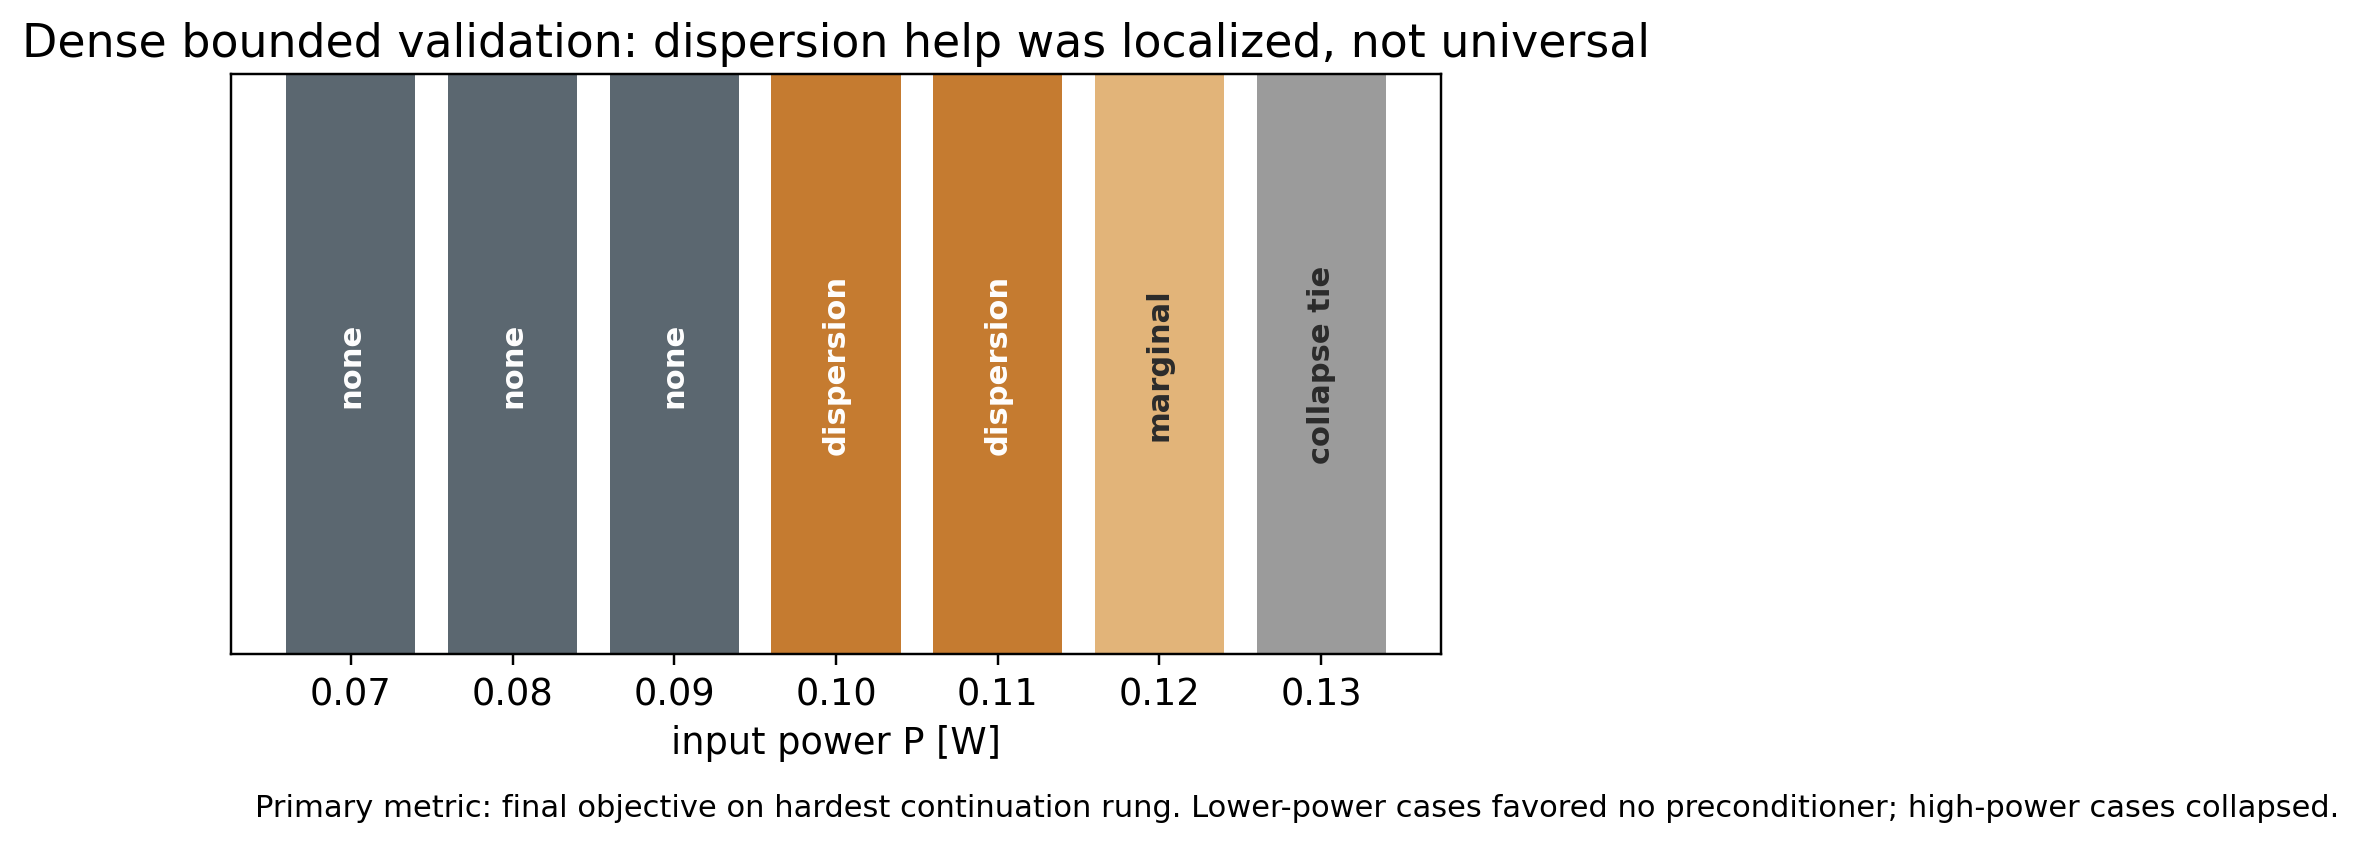
\includegraphics[width=0.86\linewidth]{figures/power_validation_regime_summary.png}
\caption{Dense bounded validation across nearby powers. The dispersion
preconditioner was not a universal win: the benefit appeared localized near a
middle-stress case and disappeared or became weak outside that window.}
\end{figure}

The follow-up power validation used the hardest continuation rung as the
primary metric. Lower-power cases favored no preconditioner. Around
\(P=0.10\,\mathrm{W}\), dispersion preconditioning gave the clearest benefit.
At higher power, both variants ran into collapse-like behavior, so a tiny
dispersion edge there is not a strong scientific result.

That is why the project-level conclusion is closure rather than expansion.
The trust-region path taught us a lot about the landscape, but it did not
produce a robust replacement for the simpler continuation-plus-L-BFGS strategy.

\subsection*{Intuition Check}

A method that wins only in a narrow setting can still be scientifically
interesting. But it should not become the default workflow. For a default
optimizer, the project needs stable wins across nearby regimes.

\section{Presentation Capsule}

If this note becomes a second-order-methods slide, the clean message is:
\begin{itemize}
    \item Trust-region Newton methods use a local quadratic model, but this Raman landscape is strongly saddle-dominated.
    \item Negative curvature is real evidence, not a plotting artifact: small gradients do not guarantee a simple minimum.
    \item Cold-start trust-region Newton did not replace L-BFGS or continuation; it mainly explained why naive second-order steps are brittle here.
    \item The presentation value of this note is diagnostic: it explains failure modes and motivates continuation, preconditioning, and careful trust checks.
\end{itemize}

\section{Lessons and Limitations}

\textbf{Lesson 1: saddle geometry is real.} Resolved Hessian spectra show both
positive and negative curvature, so a small gradient does not mean a clean
minimum.

\textbf{Lesson 2: cold-start trust-region Newton is brittle here.} The
radius-sweep result rules out the simplest explanation that the first radius
was just chosen badly.

\textbf{Lesson 3: gauge handling is not optional.} Preconditioning can push
vectors out of the gauge-complement subspace unless residuals, directions, and
final steps are re-projected.

\textbf{Lesson 4: continuation matters more than preconditioning.}
Dispersion scaling helped only after a continuation path supplied a useful
initial phase mask.

\textbf{Limitation 1: bounded cases are not final production runs.} The
preconditioning comparisons were intentionally limited. They are enough to
make a research decision, but they are not a comprehensive method paper.

\textbf{Limitation 2: HVPs are finite-difference objects.} The Hessian-vector
products depend on gradient accuracy and finite-difference step choice. They
are useful, but they are not exact symbolic Hessians.

\textbf{Limitation 3: objective scale matters.} Curvature numbers from
different objective conventions should not be mixed as if they live on the
same numerical scale. The reliable comparison is the sign pattern and the
behavior of the actual trust-region runs.

\section{Reproduction Capsule}

The trust-region utilities live under
\texttt{scripts/research/trust\_region/}. Substantial reruns should use Julia
threading and the project heavy-job workflow when the grid or sweep is large:
\[
    \texttt{julia -{}-project=. -t auto <trust-region-driver>.jl}
\]
For a complete run, the important outputs are:
\begin{itemize}
    \item trust report markdown with exit code, final objective, accepted-step
    counts, and HVP budget;
    \item telemetry CSV with per-iteration \(\rho\), radius, and step status;
    \item standard image set for each representative result:
    phase diagnostic, shaped evolution, and unshaped evolution;
    \item visual inspection of representative best, typical, failed, and
    control cases before using the result in a report.
\end{itemize}

\section{Sources and References}

\begin{thebibliography}{9}
\bibitem{agrawal2019}
G. P. Agrawal. \textit{Nonlinear Fiber Optics}, 6th ed. Academic Press, 2019.
\url{https://www.sciencedirect.com/book/9780128170427/nonlinear-fiber-optics}

\bibitem{dudley2006}
J. M. Dudley, G. Genty, and S. Coen. ``Supercontinuum generation in photonic
crystal fiber.'' \textit{Reviews of Modern Physics}, 78, 1135--1184, 2006.
\url{https://doi.org/10.1103/RevModPhys.78.1135}

\bibitem{hult2007}
J. Hult. ``A fourth-order Runge-Kutta in the interaction picture method for
simulating supercontinuum generation in optical fibers.'' \textit{Journal of
Lightwave Technology}, 25(12), 3770--3775, 2007.
\url{https://doi.org/10.1109/JLT.2007.909373}

\bibitem{liu1989}
D. C. Liu and J. Nocedal. ``On the limited memory BFGS method for large scale
optimization.'' \textit{Mathematical Programming}, 45, 503--528, 1989.
\url{https://doi.org/10.1007/BF01589116}

\bibitem{steihaug1983}
T. Steihaug. ``The conjugate gradient method and trust regions in large scale
optimization.'' \textit{SIAM Journal on Numerical Analysis}, 20(3), 626--637,
1983. \url{https://doi.org/10.1137/0720042}

\bibitem{nocedal2006}
J. Nocedal and S. J. Wright. \textit{Numerical Optimization}, 2nd ed.
Springer, 2006. \url{https://link.springer.com/book/10.1007/978-0-387-40065-5}

\bibitem{conn2000}
A. R. Conn, N. I. M. Gould, and P. L. Toint. \textit{Trust Region Methods}.
SIAM, 2000. \url{https://doi.org/10.1137/1.9780898719857}

\bibitem{morales2000}
J. L. Morales and J. Nocedal. ``Automatic preconditioning by limited memory
quasi-Newton updating.'' \textit{SIAM Journal on Optimization}, 10(4),
1079--1096, 2000. \url{https://doi.org/10.1137/S1052623497327854}
\end{thebibliography}

\end{document}
